\colorlet{chaptergrey}{red!60!yellow!30!}
\chapter[Spin and the cosmic web]{Exploring the role of the cosmic web in galaxy evolution using kinematics}
\label{ch:halo_assembly}
\vspace{-5.25in}
\includegraphics[height=1.21in]{thesis/latex/headers/ifu_cw.pdf}
\vspace{3in}

\epigraph{This chapter is partially based on Kraljic, Duckworth, Tojeiro et al. (in prep.) and Duckworth, Tojeiro, Kraljic, Sgr\'o, Wild, Weijmans, Lacerna and Drory, in MNRAS, 448, Issue 1, 2019. Here, we investigate how large scale IFS surveys can be utilized to understand the relationship between galaxy kinematics and their large-scale environment.}

\section{Introduction}
In Chapters 2 and 3, we demonstrated how galaxy kinematics are closely related to morphological properties, baryonic processes such as AGN feedback, and the characteristics of its surrounding dark matter halo. The stellar (dark matter halo) mass of a galaxy encodes a lot of its evolution, demonstrating that \textit{local environment} (and over-density) can explain a large part of the diversity of properties we observe.

As introduced in \S\ref{sec:cosmic_web_intro}, galaxies on large scales are organised within the cosmic network of filamentary structure. Dark matter haloes and their constituent galaxies are subject to the large-scale anisotropic forces throughout their formation and evolution, in particular shaping their initial angular momentum content, before non-linear baryonic processes take hold. There is growing evidence that the cosmic web environment of a galaxy, also plays a significant role in galaxy evolution and is, at least partially, driving their morphology. 

Revisiting tidal torque theory \citep[TTT; e.g.][]{hoyle1951, peebles1969} in the context of large-scale anisotropic environment, \citet{codis2015} explain the relative angular momentum distribution of haloes with respect to neighbouring filaments and walls. The misalignment between the inertia tensors of the proto-haloes and the directionality of the tidal tensor due to the neighbouring wall or filament leads to a spin alignment for low mass haloes. As these haloes grow in mass hierarchically, merging with other haloes and they lose this preferential alignment with large scale structure. Due to the flow of matter along walls and filaments, mergers often happen in this plane, possibly leading to a \textit{flip} in direction, so that higher mass dark matter haloes are preferentially perpendicular to the orientation of the tidal field \citep[e.g.][]{Codis2012, dubois2014, GaneshaiahVeena2018}. This understanding is motivated by cosmological N-body simulations and learning how this propagates to observations is complex. In simulations, the constituent galaxies appear to retain a memory of the spin orientation (with respect to large scale structure) as dictated by their host dark matter halo \citep[e.g.][]{codis2018, Kraljic2019flip}. The mass dependence of the spin alignment \textit{flip} is, however, debated and likely dependent on different choices for baryonic processes and the scale of the neighbouring filamentary structure. The orientation of galaxies with respect to large-scale structure is, however, only one aspect in determining the relationship between galaxy evolution and the cosmic web. In this theoretical framework, it could be expected that not only the spin alignment, but also, the spin \textit{magnitude} of a given galaxy would be modulated as function of its position within the cosmic web.

A powerful approach in a holistic understanding of galaxy evolution, and hence, potentially enabling us to trace the impact of the cosmic web, is spatially resolved spectroscopy. As introduced in \S\ref{sec:ifs_surveys_intro} IFS surveys for thousands of galaxies, across a wide variety of morphologies, environments, and masses in the local Universe are now a reality. Current generation IFS surveys such as MaNGA and SAMI have opened the door for a detailed understanding between kinematics, morphology, and, stellar mass ($\mathrm{M_{stel}}$). Using data from the SAMI IFS survey, \citet{cortese2016} demonstrated that the angular momentum of both stars and gas correlates strongly positive with stellar mass. For galaxies with $\mathrm{M_{stel} > 10^{9.5} M_{\odot}}$, the scatter in the $\mathrm{M_{stel}}$ - angular momentum relationship can be constrained by optical morphology (i.e. sersic index). This scatter, however, can be even more strongly correlated with $\mathrm{\lambda_R}$ (as defined in equation \ref{eq:lambda_R}; here only calculated within 1\re). These tight relationships indicate that early-type fast rotators and late-type galaxies are not two separate classes of objects, but represent a `continuum' connecting pure-disks to bulge-dominated systems. In MaNGA, \citet{graham2018} investigate the relationship between angular momentum and optical morphology for $\sim$2300 galaxies. They demonstrate that both stellar mass and morphology correlate strongly with the stellar angular momentum of galaxies. Furthermore, they use $\mathrm{\lambda_R}$ and ellipticity to separate early-type galaxies into fast and slow rotators, finding a clear bi-modality in their distribution, and hence, potentially highlighting their different assembly histories. 

The relationship between stellar angular momentum and environment in observations is, however, less clear. In MaNGA, \citet{greene2018} make use of the \citet{yang2007} group catalogue (introduced in \S\ref{sec:group_def}) to define halo mass and separate galaxies into central and satellites. They find minimal evidence that $\mathrm{\lambda_R}$ / $\epsilon^{0.5}$ (i.e. stellar angular momentum normalised by shape) depends on the mass of the group, once the role of $\mathrm{M_{stel}}$ has been accounted for. They also find minimal difference between centrals and satellites, in terms of slow rotator fraction. \citet{wang2020} demonstrate that the environmental dependence of stellar angular momentum is significantly weaker than the stellar mass dependence. While there is no particular trend with halo mass for low mass galaxies, high mass ($\mathrm{M_{stel} > 10^{10.9} M_{\odot}}$) central galaxies (or those in dense/rich groups) have lower $\mathrm{\lambda_R}$. Extending this idea, \citet{graham2019} use 3900 galaxies in MaNGA to demonstrate that the fraction of galaxies defined as slow rotator \textit{does} increase with overdensity, however, there is a more marked effect when comparing to the relative density (i.e. correlating with the relative peak densities, rather than absolute which averages signal out). Even further, using distance to cluster/group centre shows the strongest trends with slow rotator fraction, suggesting a direct link with SR creation (from dry merger events and are selected to be $\mathrm{M_{stel} > 2\times10^{11} M_{\odot}}$) and cluster cores. This holds true at fixed stellar mass ($\mathrm{M_{stel} > 2\times10^{11} M_{\odot}}$). How the spin magnitude of galaxies is modulated by \textit{large-scale} environment, however, is a topic in its infancy at the time of writing (observationally). In this chapter, we use the MaNGA survey to explore two questions:

\begin{itemize}
    \item How does the magnitude of stellar angular momentum in galaxies depend individually on morphology, stellar mass, halo mass, and, cosmic environment?
    \item Does the spin orientation of galaxy disks in the local Universe align with the local geometry of neighbouring filaments?
\end{itemize}

In \S\ref{sec:spin_magnitude} we investigate how the stellar angular momentum content of galaxies in MaNGA is dependent on local and large-scale environment. We make use of the largest IFS galaxy sample to date (MPL-9; exactly 8000 unique galaxies before cross-matching), to understand how galaxy spin is modulated with respect to different morphological features of the cosmic web once stellar mass, and, morphology have been accounted for. We also consider how group membership and halo mass can drive individual changes in the angular momentum content. In \S\ref{sec:spin_alignment} we present the first study making use of galaxy kinematics to estimate the 3D alignment between the spin direction of galaxy disks and their neighbouring filamentary structure. We investigate the dependence of spin alignment on stellar mass and galaxy morphology, to better understand the connection between galaxy evolution and the cosmic web. We summarise and conclude in \S\ref{sec:cw_spin_conclusion}.

\section{Data and Methods}
\subsection{Galaxy sample} \label{sec:spin_galaxy_sample}
In \S\ref{sec:spin_magnitude}, we base our analysis on 8000 unique galaxies corresponding to the 9th MaNGA product launch. In contrast, we make use of 4633 unique galaxy observations (MPL-6) for \S\ref{sec:spin_alignment}, reflecting the state of the survey as of mid-2018 (data released publicly December 2018). MPL-6 is also our defined sample in the following chapter. As in Chapters 2 and 3, stellar mass estimates are taken from elliptical petrosian fits from the NSA catalogue, used as a target sample for MaNGA. 

\subsection{DisPerSE} \label{sec:disperse_sdss}
For all work in this chapter (and Chapter 5), we characterise the topological features of the cosmic web using the Discrete Persistent Structure Extractor Code \citep{sousbie2011a, sousbie2011b} as introduced in \S\ref{sec:cosmic_web_intro}. Here DisPerSE is applied to a modified version of the SDSS DR10 spectroscopic sample as described in \citet{tempel2014}. In observations, there is an additional difficulty since we are not working with exact three dimensional positions in real space, but rather, in redshift space. To recover the intrinsic galaxy position, an estimation for the peculiar velocity must be made for each galaxy. On large-scales this corresponds to the Kaiser effect \citep{kaiser1987}, which acts to increase the contrast of the skeleton due the coherent motion of galaxies with the growth of structure \citep[e.g.][]{shi2016}. On small-scales, however, the Fingers of God effect \citep[FOG;][]{jackson1972,tulley1978} derives from random motions of galaxies within virialized haloes. The latter can elongate structure in redshift space leading to erroneous identification of filaments. We correct for the FOG effect using the technique outlined in \citet{kraljic2018}. As introduced in \S\ref{sec:cosmic_web_intro}, the \textit{robustness} of the cosmic web's morphological features identified are quantified using the so called persistence ratio, a measure of the significance of the topological connection between individual pairs of critical points. Here we use choose robust filaments identified with a significance of 5$\sigma$. In Figure \ref{fig:disperse_sdss} we show an example of the recovered density field from the set of galaxy positions in SDSS and the corresponding ridge extraction (i.e. filament detection). \red{length of typical segments with respect to typical distance to galaxy?}

\begin{figure*}
    \centering
	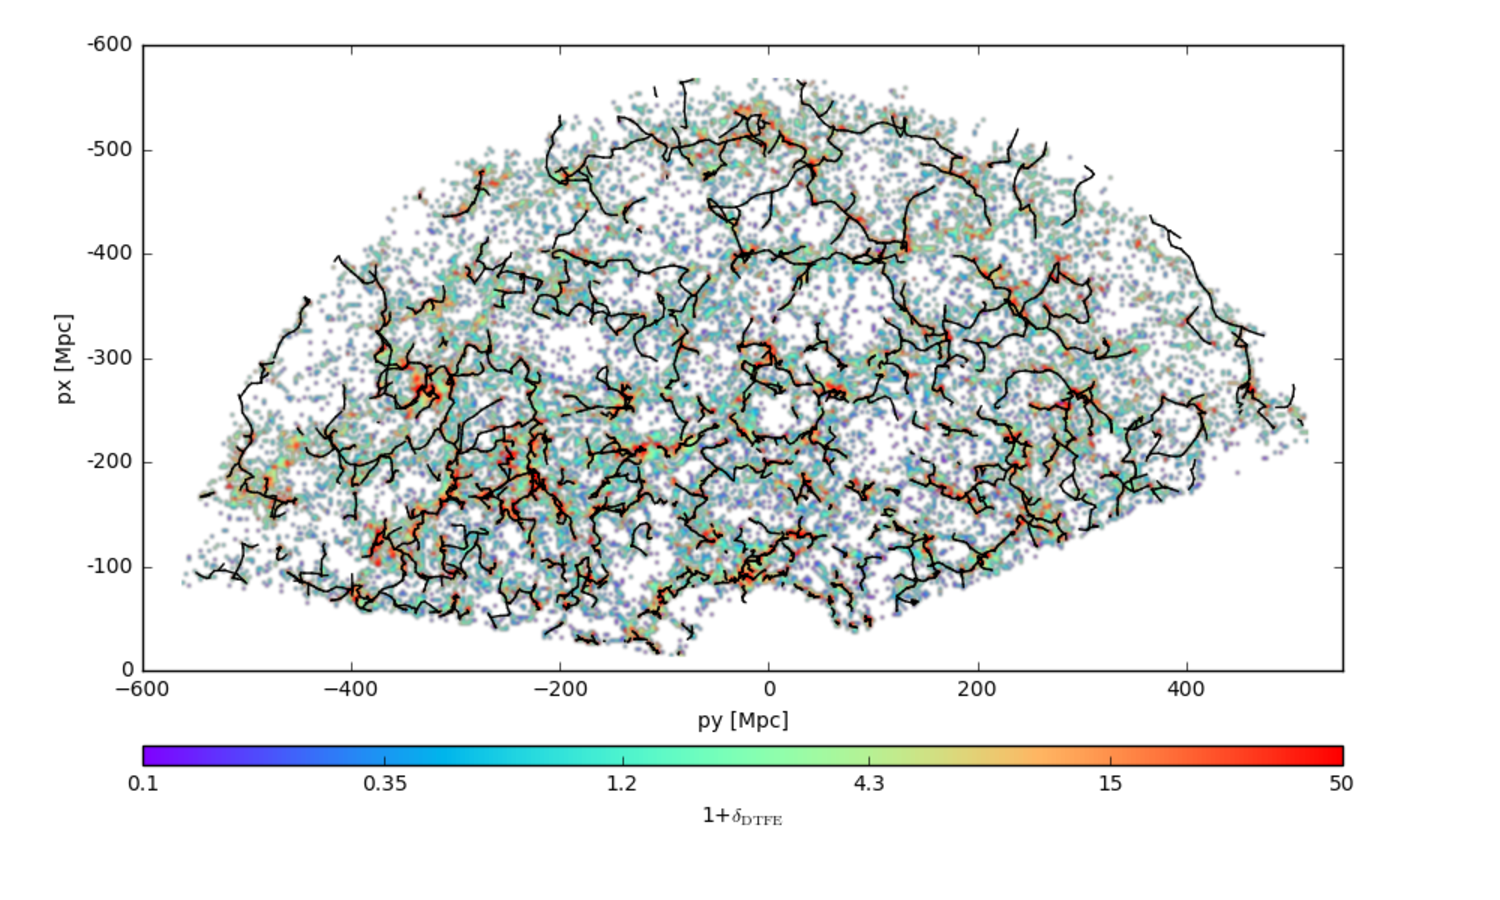
\includegraphics[width=\linewidth]{thesis/latex/halo_assembly_manga/SDSS_CW_DisPerSE.pdf}
    \caption[Illustration of the filamentary network for a slice of the SDSS field.]{Illustration of the filamentary network (black lines) for a slice of the SDSS field ($0.02 \leq z \leq 0.15$; $ 27 \leq$ dec $\leq 33$) extracted using the DisPerSE code. Only filamentary structures which are seen to persist above the 5$\sigma$ threshold are shown, along with the density contrast of the galaxy population. The density contrast is estimated using the small-scale DTFE estimator (see text). Adapted from \citet{duckworth2019_halo}, with credit to K. Kraljic.}
    \label{fig:disperse_sdss}
\end{figure*}

The local geometry of each filament is characterised by a series of smaller \textit{segments}, which are the default output of the DisPerSE code. For each galaxy, the nearest segment is found and its direction is used to compare to the given galaxy's spin direction. 

\subsubsection{Cosmic web distances} \label{sec:cosmic_web_distances}
Having constructed a skeleton of the cosmic web, a galaxy's environment can be described by finding its vicinity to various features of the skeleton. The cosmic web comprises of low density `void' regions which are enclosed by `walls' of structure which become filaments at points of intersection. The gravitational potential of the filaments dictate the flow of the matter, which at the point of intersection, feed high density regions interpreted as `nodes'. Along the filament, saddle points remain as minima between the flows towards nodes. A schematic for the distances to morphological features of the cosmic web is given in Figure \ref{fig:disperse_schematic}. 

\begin{figure}
    \centering
	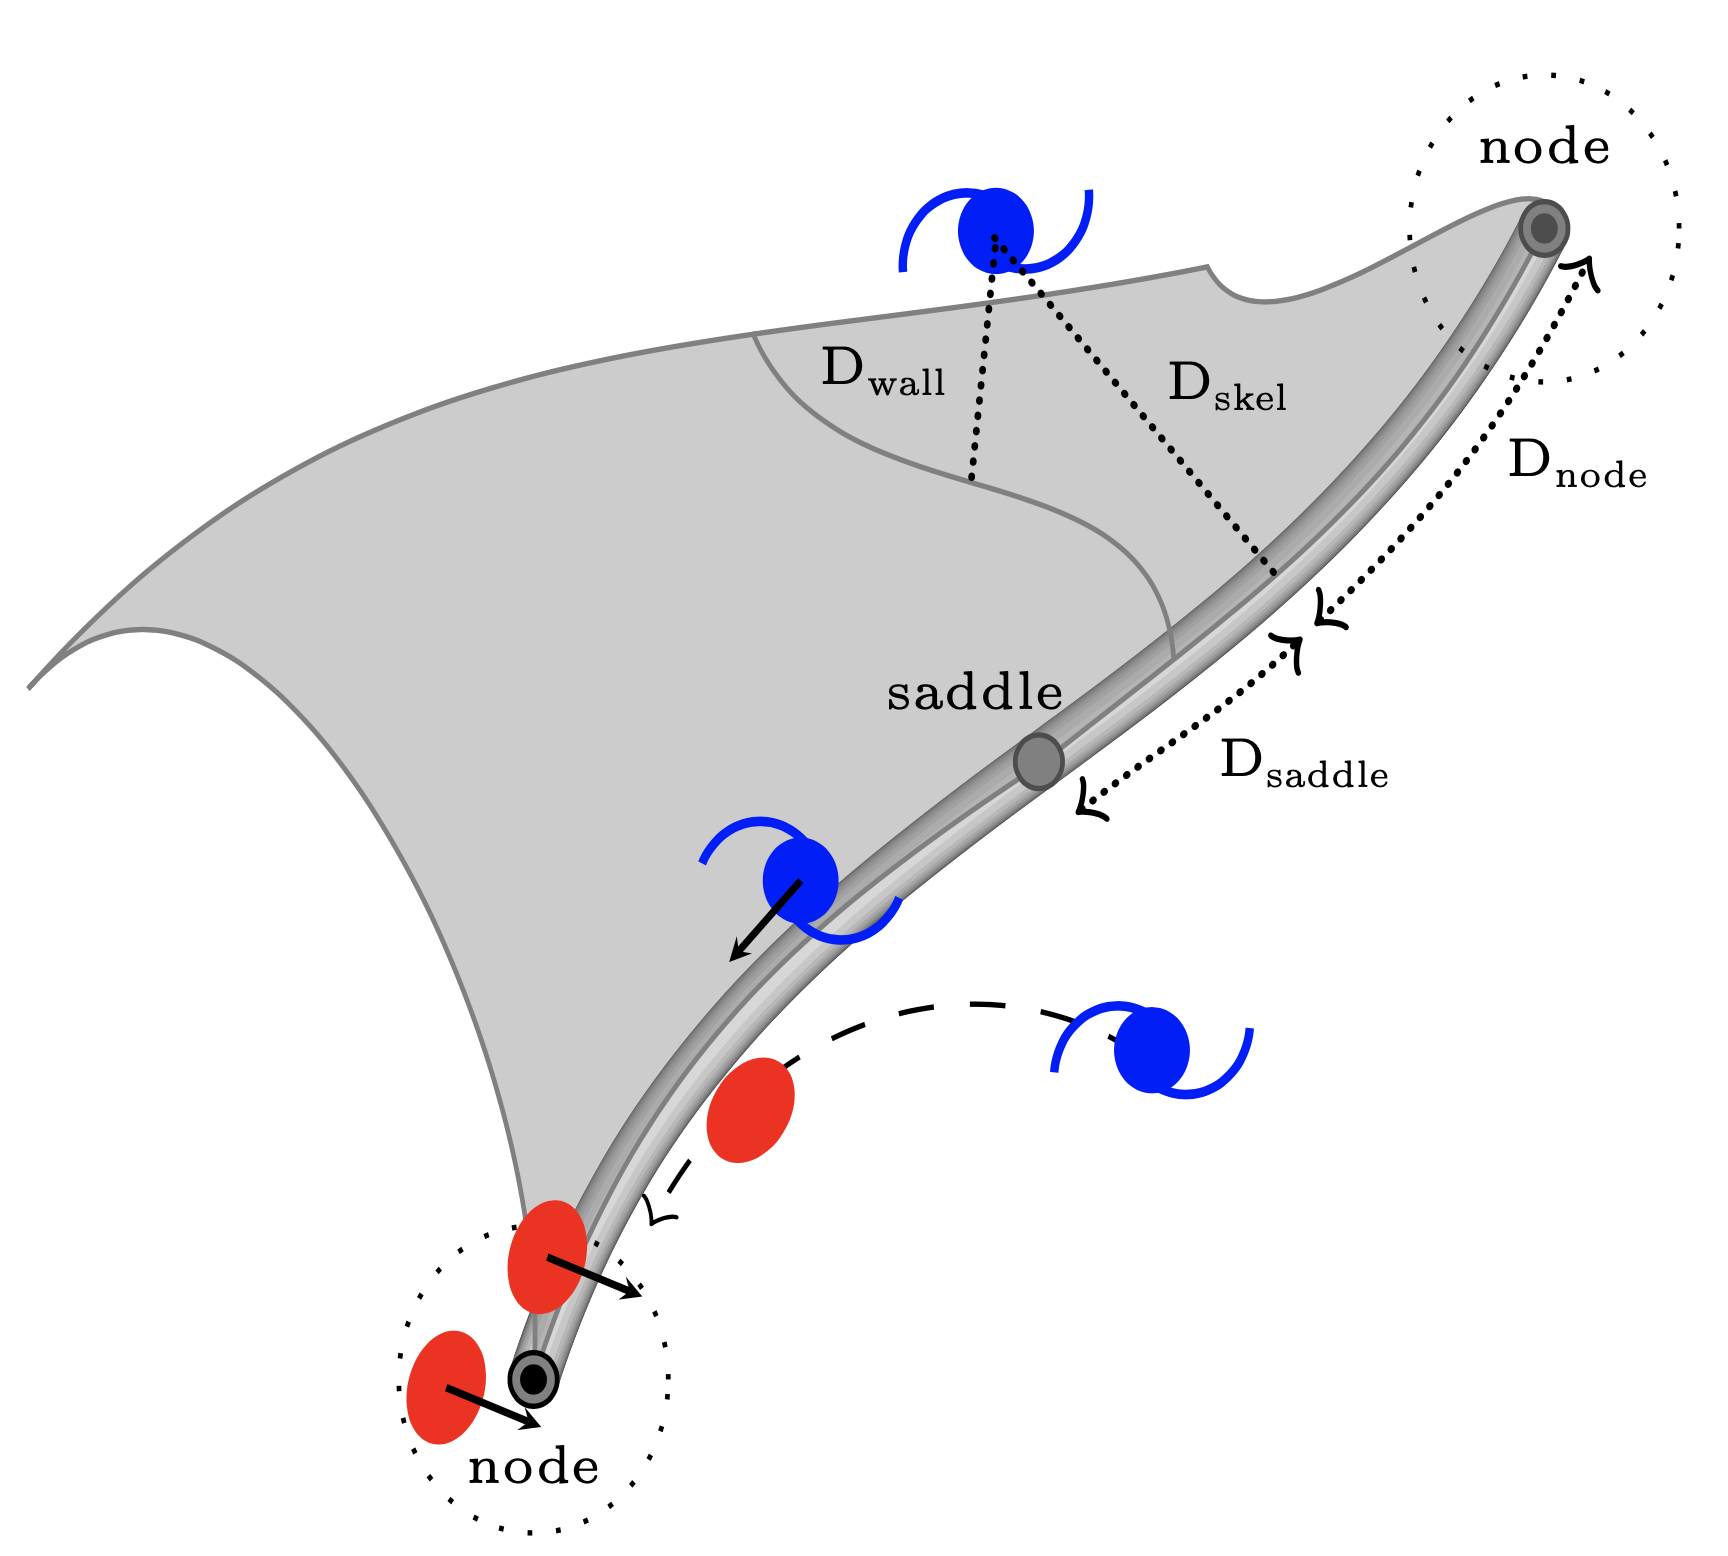
\includegraphics[width=0.5\linewidth]{thesis/latex/cw_spin/cw_disperse_diagram.png}
    \caption{Schematic view of the cosmic web as identified in the framework of DisPerSE. The position of a given galaxy is parametrised by its distance to the nearest filament ($D_{skel}$), and it distance to the nearest wall ($D_{wall}$). $D_{node}$ and $D_{saddle}$ represent the distances from the impact point to the node and saddle along the corresponding filament, respectively (i.e. maxima and minima along the filament). Taken from \citet{kraljic2018}.}
    \label{fig:disperse_schematic}
\end{figure}

The distance to the nearest filamentary point, $D_{skel}$, is first found for each galaxy. To then consider the influence of the nearest node, the distance from this impact point along the filament to the node is also computed, $D_{node}$. Finally the distance to the nearest wall, $D_{wall}$, can then be found. In order to investigate expected trends of galaxies with vicinity to any cosmic web feature we must remove effects resulting due to the proximity of others. For $D_{skel}$ we remove all galaxies that lie within $D_{node} < 0.5$ Mpc. This represents a compromise between eliminating the effect of other cosmic web features and having enough galaxies left to construct a statistically significant sample. Tightening the condition with respect to nodes so that we require $D_{node} > 1$ Mpc does not change any of the results presented in this work. 

For the purpose of \S\ref{sec:spin_alignment} only, to increase the statistics of the measured signal, each galaxy is associated with its two closest filaments. There is an absolute cut-off in distance for galaxies to be associated with a given filament; $\leq$ 13 Mpc, which represents a compromise between a clean and sufficiently large sample. As expected, including galaxies that are at very large distances from the filamentary network or that are in the highest density regions, typically galaxy groups and clusters, decreases the strength of the signal.

Construction of the cosmic web from any observation is influenced by the completeness and the sampling of the galaxy sample. The modified SDSS DR10 spectroscopic sample is complete to $m_r$ = 17.77. A sample containing only brighter galaxies will naturally only identify stronger/larger filamentary features and hence smaller substructures will be missed. In addition, the lower the sampling of galaxies, the lesser the accuracy of the actual position of cosmic web features. To correct for this, the distances are normalised by the mean inter-galaxy separation, $\left\langle D_z \right\rangle$ at a given redshift, as such $\left\langle D_z \right\rangle = n(z)^{-1/3}$ where $n(z)$ is the number density. \red{rewrite this paragraph}

\section{Spin magnitude} \label{sec:spin_magnitude}
In this section, we use 8000 galaxies from the MaNGA survey to clearly demonstrate the relationship between stellar angular momentum ($\mathrm{\lambda_R}$), stellar mass, and, morphology in the context of previous work. This sets the foundation for understanding how $\mathrm{\lambda_R}$ correlates with more subtle properties such as halo mass, group membership, and, vicinity to morphological features of the cosmic web.

\subsection{Morphology}
Throughout this chapter, we select our sample based on the visual morphological classifications of GalaxyZoo2 \citep[GZ2][]{willett2013} as introduced in \S\ref{sec:morph_def_obs}. For the purpose of \S\ref{sec:spin_magnitude}, we select the same vote thresholds as chapter 2 (i.e. $P = 0.7$ for a given morphological feature). Lenticulars (i.e. in this instance a broad S0-Sa classification) are again selected by Equation 19 of \citet{willett2013}. In this section we also include a category of `unclassified' galaxies; i.e. those not associated with any particular morphological group.

Figure \ref{fig:morph_lambdaR_mstel} shows the distribution of $\mathrm{\lambda_R}$ as a function of stellar mass ($\mathrm{M_{stel}}$) for each morphological classification; ETGs (red), LTGs (navy) and unclassified (orange). LTGs are separated further into S0-Sas (green) and Sb-Sds (light blue). In each panel, the distribution of each sample is represented by a kernel density estimator (KDE) that smooths the discrete galaxy positions in the phase space into contours. A binned mean of $\mathrm{\lambda_R}$ as function $\mathrm{M_{stel}}$ is overlaid with errorbars representing standard error on the mean. As expected, for all galaxies (left panel), there is a clear trend going from early-type to late-type of higher $\mathrm{\lambda_R}$, regardless of stellar mass. For each morphological category, there is a general trend that $\mathrm{\lambda_R}$ decreases with stellar mass. 

We also separate our sample by group membership using the \citep{lim2017} group catalogue (introduced in \ref{sec:group_def}). We separate our galaxies into centrals and satellites, along with an assigned halo mass for the group based on the total contained stellar mass. After cross-matching we find that around $\mathrm{2/3^{rds}}$ of our sample are centrals, hence explaining why the middle panel (centrals only) is broadly consistent with the left hand side (all galaxies). For the satellites (right panel) we find that the distinct trends with stellar mass, regardless of morphology, is slightly suppressed. In particular, there is only a small decrease in $\mathrm{\lambda_R}$ with increasing stellar mass for the LTGs.

\begin{figure}
    \centering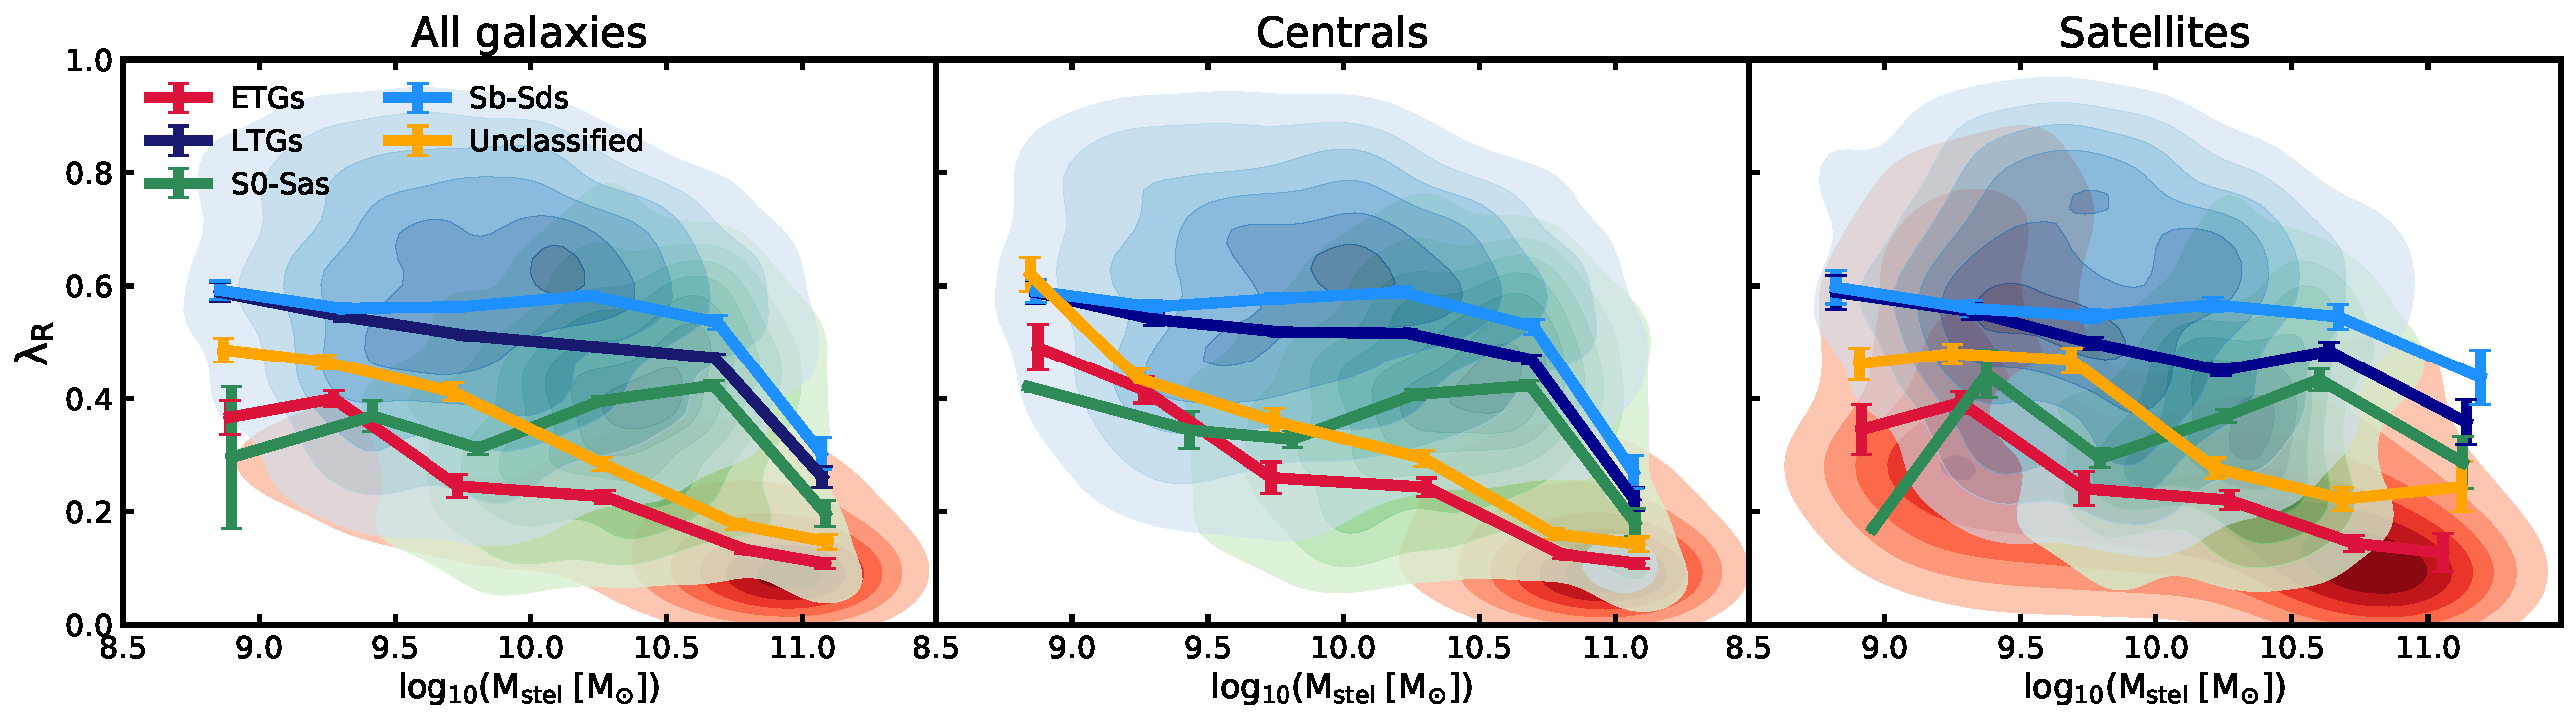
\includegraphics[width=\linewidth]{thesis/latex/cw_spin/morphology_lambdaR_mstel_kde_wo_unclassified.pdf}
    \caption{Distribution of stellar angular momentum ($\mathrm{\lambda_R}$) as a function of stellar mass ($\mathrm{M_{stel}}$) for all ETGs (red), LTGs (dark blue), S0-Sas (green), Sb-Sds (light blue) and unclassified (orange) in MaNGA. The panels (left to right) shows the distributions for all galaxies, centrals only and satellites only respectively. In each panel, the overall distribution for ETGs, S0-Sas and Sb-Sds is shown by the contours using a KDE (see text), with average $\mathrm{\lambda_R}$ values shown in bins of $\mathrm{M_{stel}}$. For all galaxies there is distinct trend with morphology and $\mathrm{\lambda_R}$  with later types being higher angular momentum than earlier types at all masses. There is also a correlation between $\mathrm{\lambda_R}$  and $\mathrm{M_{stel}}$ for each morphological type, with galaxies at higher mass typically having lower angular momentum.}
\label{fig:morph_lambdaR_mstel}
\end{figure}

We now investigate the angular momentum evolution with respect to halo mass for these sub-populations in Figure \ref{fig:morph_lambdaR_mhalo}. Again galaxy morphology population is shown by a KDE (not shown for the unclassified objects which cover most of the phase space) along with a binned mean of $\mathrm{\lambda_R}$ as function $\mathrm{M_{halo}}$. Regardless of stellar or halo mass, the trends seen in previous work remain clear here: \textit{$\mathrm{\lambda_R}$ increases with later galaxy morphologies.} ETGs (which appears to be driven by centrals) show a similar evolution as with stellar mass, with $\mathrm{\lambda_R}$ decreasing with increasing $\mathrm{M_{halo}}$. S0-Sas and Sb-Sds have relatively flat distributions of $\mathrm{\lambda_R}$ as a function of halo mass, however, the combined populations (LTGs) shows a similar slight decrease as with $\mathrm{M_{stel}}$. One marked difference with the halo mass distributions is the lack of sudden drop towards high masses for the later types (with respect to stellar mass). The most massive LTGs appear to be significantly lower spin, whereas, those galaxies in the most massive haloes have only marginally lower $\mathrm{\lambda_R}$ values. Regardless of morphology, the environmental dependence for satellite galaxies (right panel) appears to be far less significant than for centrals (middle panel). 

\begin{figure}
    \centering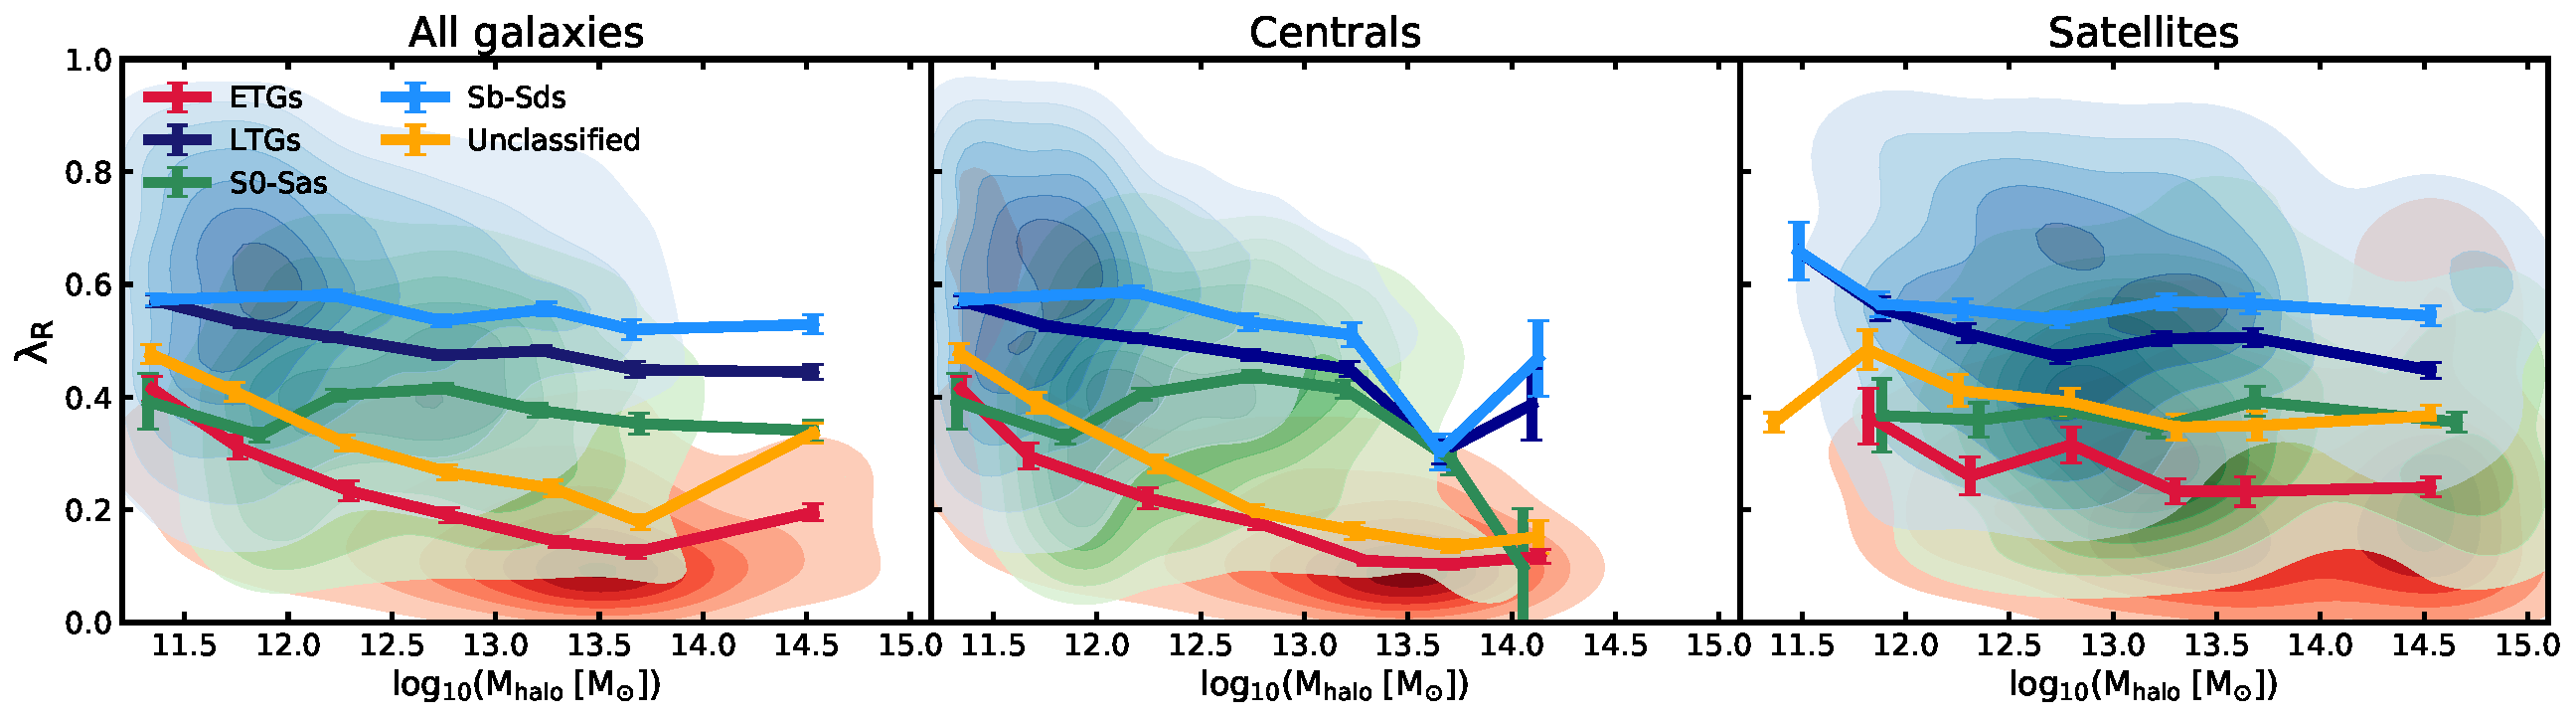
\includegraphics[width=\linewidth]{thesis/latex/cw_spin/morphology_lambdaR_mhalo_kde_wo_unclassified.pdf}
    \caption{Distribution of stellar angular momentum ($\mathrm{\lambda_R}$) as a function of halo mass ($\mathrm{M_{halo}}$) for all ETGs (red), LTGs (dark blue), S0-Sas (green), Sb-Sds (light blue) and unclassified (orange) in MaNGA. The panels (left to right) shows the distributions for all galaxies, centrals only and satellites only respectively. In each panel, the overall distribution for ETGs, S0-Sas and Sb-Sds is shown by the contours using a KDE (see text), with average $\mathrm{\lambda_R}$ values shown in bins of $\mathrm{M_{halo}}$. For all galaxies there is distinct trend with morphology and $\mathrm{\lambda_R}$  with later types being higher angular momentum than earlier types at all masses. There is also a correlation between $\mathrm{\lambda_R}$ and $\mathrm{M_{halo}}$ for each morphological type, with galaxies in higher mass haloes typically having lower angular momentum. The trend is far weaker than with respect to stellar mass, however.}
\label{fig:morph_lambdaR_mhalo}
\end{figure} 

\subsection{Group membership}
To better visualise how $\mathrm{\lambda_R}$ is individually dependent on group membership, in Figure \ref{fig:group_membership_lambdaR} we plot the overall central (navy) and satellite (green) galaxy populations as a function of stellar mass (left panel) and halo mass (right panel). In each panel, the distribution of central and satellites are shown by KDEs along with binned mean as a function of stellar (halo) mass respectively. In addition the binned mean for all galaxies is shown in black, with all errorbars computed by standard error on the mean. For all galaxies, we find a clear difference between the dependence of $\mathrm{\lambda_R}$ on stellar and halo mass. As seen for the individual morphologies in Figure \ref{fig:morph_lambdaR_mstel}, $\mathrm{\lambda_R}$ decreases steadily with increasing stellar mass with a sharp drop off for $\mathrm{M_{stel} > 10^{10.5}M_{\odot}}$. While $\mathrm{\lambda_R}$ decreases steadily with $\mathrm{M_{halo}}$, in contrast to stellar mass, there is no sharp drop off at the highest halo masses. 

Now considering centrals and satellites individually, we find that both are statistically consistent as a function of $\mathrm{M_{stel}}$. In contrast, there is marked difference with satellites having higher stellar angular momentum in haloes with $\mathrm{M_{halo} > 10^{12.5}M_{\odot}}$ in comparison to centrals, which increases with mass. This is likely a result of the distinct trend with stellar mass. The largest groups will also host the most massive central galaxies (i.e. those with $\mathrm{M_{stel} > 10^{10.5}M_{\odot}}$), which leads to a clear decrease in $\mathrm{\lambda_R}$. In general the $\mathrm{\lambda_R}$ evolution with $\mathrm{M_{halo}}$ for satellite galaxies is flatter, highlighting the limited impact of environment. Stellar mass appears to encapsulate this behaviour completely with $\mathrm{\lambda_R}$ value regardless of group membership.

\begin{figure}
    \centering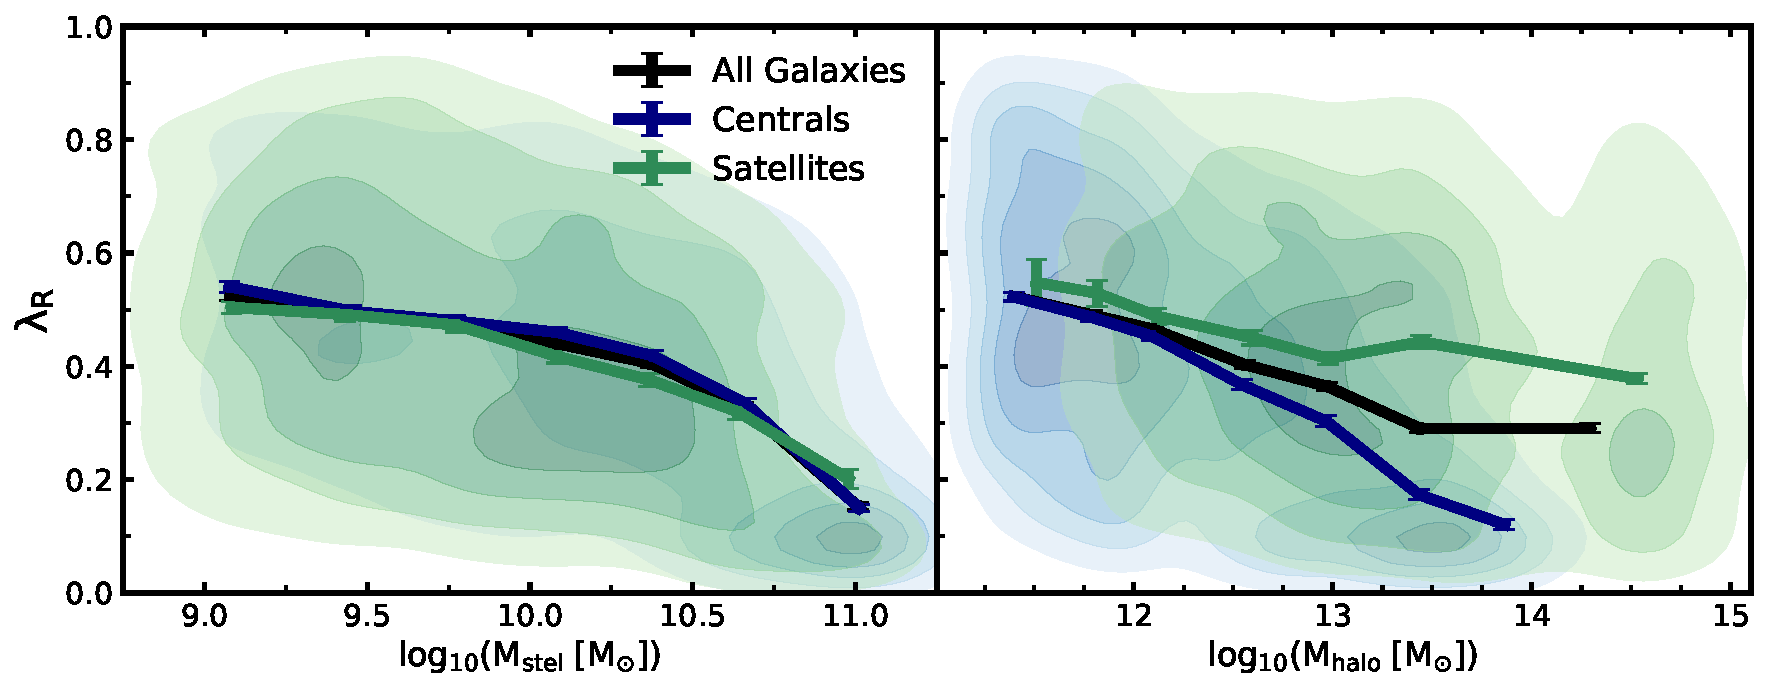
\includegraphics[width=\linewidth]{thesis/latex/cw_spin/group_lambdaR_mstel_mhalo_comparison.pdf}
    \caption{Left (right): Distribution of stellar angular momentum ($\mathrm{\lambda_R}$) as a function of stellar (halo) mass. In each panel, the overall distribution for centrals (navy) and satellites (green) are shown by the contours using a KDE (see text), with average $\mathrm{\lambda_R}$ values shown in bins of stellar (halo) mass. The average for the all galaxies is also shown in black. There is no statistical difference between centrals and satellites when plotting $\mathrm{\lambda_R}$ as a function of stellar mass, however, there is a distinct difference when going to higher halo masses.}
\label{fig:group_membership_lambdaR}
\end{figure} 

\subsection{Cosmic web}
As highlighted in \citep{graham2019}, the formation of massive slow rotating galaxies likely happens in tandem with the formation of the density peaks within groups. To better understand how environment impacts a galaxy's angular momentum content, we now investigate how $\mathrm{\lambda_R}$ is modulated by distance to different morphological features of the cosmic web. Here, we use the geometric ridge extractor DisPerSE (see \S\ref{sec:disperse_sdss}) to find the distance to nodes (i.e. maxima of the density field) and filaments for each galaxy. In Figure \ref{fig:lambdaR_dnode}, we show the distribution of $\mathrm{\lambda_R}$ as function of distance to nodes (i.e. peaks in the density field; $D_{node}$). In each panel, galaxies are split into three populations; $\mathrm{M_{stel} \leq 10^{9.7}M_{\odot}}$ (green), $\mathrm{10^{9.7}M_{\odot} < M_{stel} < 10^{10.4}M_{\odot}}$ (orange) and $\mathrm{M_{stel} \geq 10^{10.4}M_{\odot}}$ (purple). Each population contains 1/3 of the total galaxy sample. 

We find that $\mathrm{\lambda_R}$ is effectively agnostic to $D_{node}$ for the low and intermediate mass populations in all panels (left-right: all galaxies, centrals, satellites). However, we find that the high mass bin does show a dependence on $D_{node}$, with the galaxies closest to nodes having lower angular momentum. This only seen for central galaxies, with high mass satellites also agnostic to vicinity to nodes. This highlights the formation and evolution of massive slow rotating central galaxies. This appears to corroborates the findings of \citet{graham2019}, that the formation of massive slow rotators happens \textit{in tandem} with the peak density within a group/cluster. This is likely a result of dry mergers which lead to the lowered angular momentum content of centrals. Interestingly we do not find the same trend for high mass satellites with respect to $D_{node}$ which is near agnostic to $D_{node}$. This again could suggest that the formation of massive slow rotating centrals happen with the formation of the density peaks themselves. While massive satellites can reside close to the density peaks, it doesn't necessitate they are of lower spin, and hence have undergone the same physical transformation.

\begin{figure}
    \centering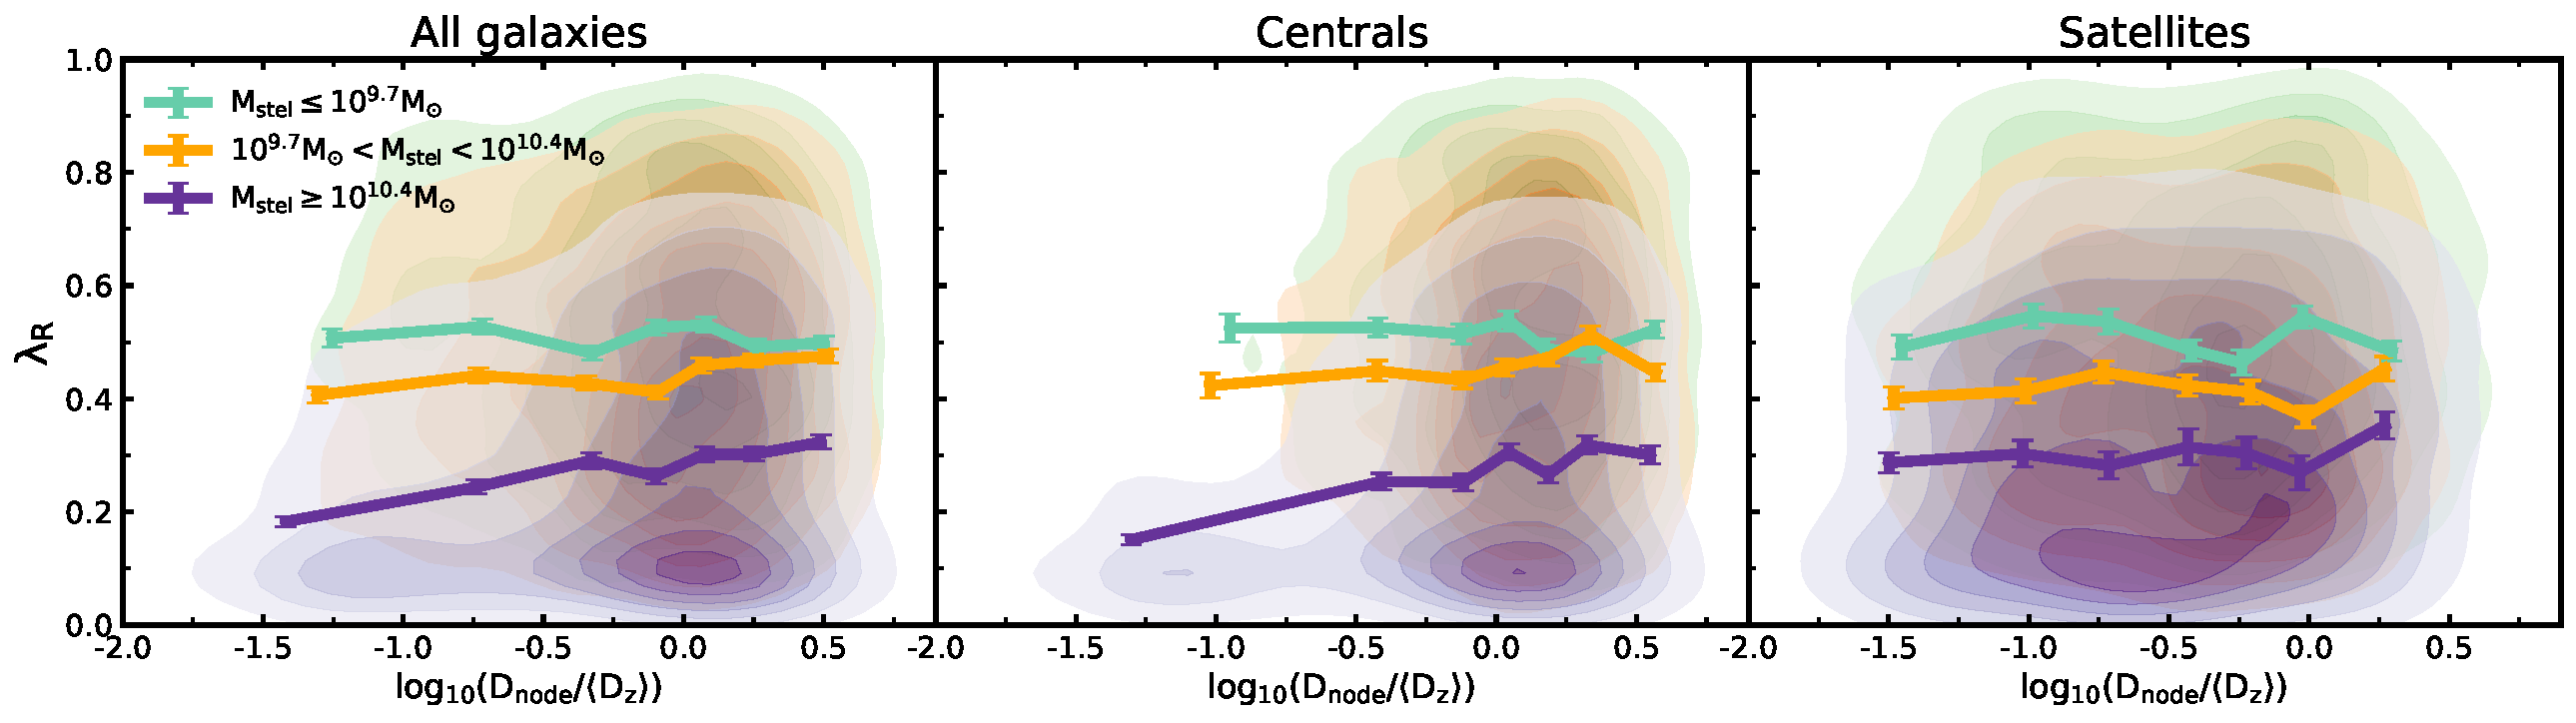
\includegraphics[width=\linewidth]{thesis/latex/cw_spin/lambdaR_dnode_mass_split_3sigma.pdf}
    \caption{Distribution of stellar angular momentum ($\mathrm{\lambda_R}$) as a function of distance to nodes ($D_{node}$). In each panel the overall distribution for three mass bins; $\mathrm{M_{stel} \leq 10^{9.7} M_{\odot}}$, $\mathrm{10^{9.7}M_{\odot} < M_{stel} < 10^{10.4}M_{\odot}}$, $\mathrm{M_{stel} \geq 10^{10.4}M_{\odot}}$ (green, orange and purple respectively) are shown by the contours using a KDE (see text), with average $\mathrm{\lambda_R}$ values shown in bins of $D_{node}$. For the low and middle mass bins, there is no particular trend with vicinity to nodes, however, the high mass bin does decrease in spin for those closer to nodes. This trend appears to be driven by centrals.}
\label{fig:lambdaR_dnode}
\end{figure} 

In the top row of Figure \ref{fig:lambdaR_dskel}, we now investigate how $\mathrm{\lambda_R}$ is dependent on distance to nearest filament ($D_{skel}$) for the three mass bins. Similar to distance to nearest node, there are no distinct trends for the low and intermediate mass bins with respect to $D_{skel}$. However, the high mass bin (i.e. $\mathrm{M_{stel} > 10^{10.4}M_{\odot}}$) we find that galaxies closer to filamentary structure, are preferentially lower angular momentum with respect to those at larger $D_{skel}$. This signal is driven by central galaxies, with high mass satellites not showing the same trend. By construction, in geometric identifications of the cosmic web all filaments start and end in nodes. Because of this, any signal found for $D_{skel}$ could be a secondary signal due to the correlation with $D_{node}$. 

\begin{figure}
    \centering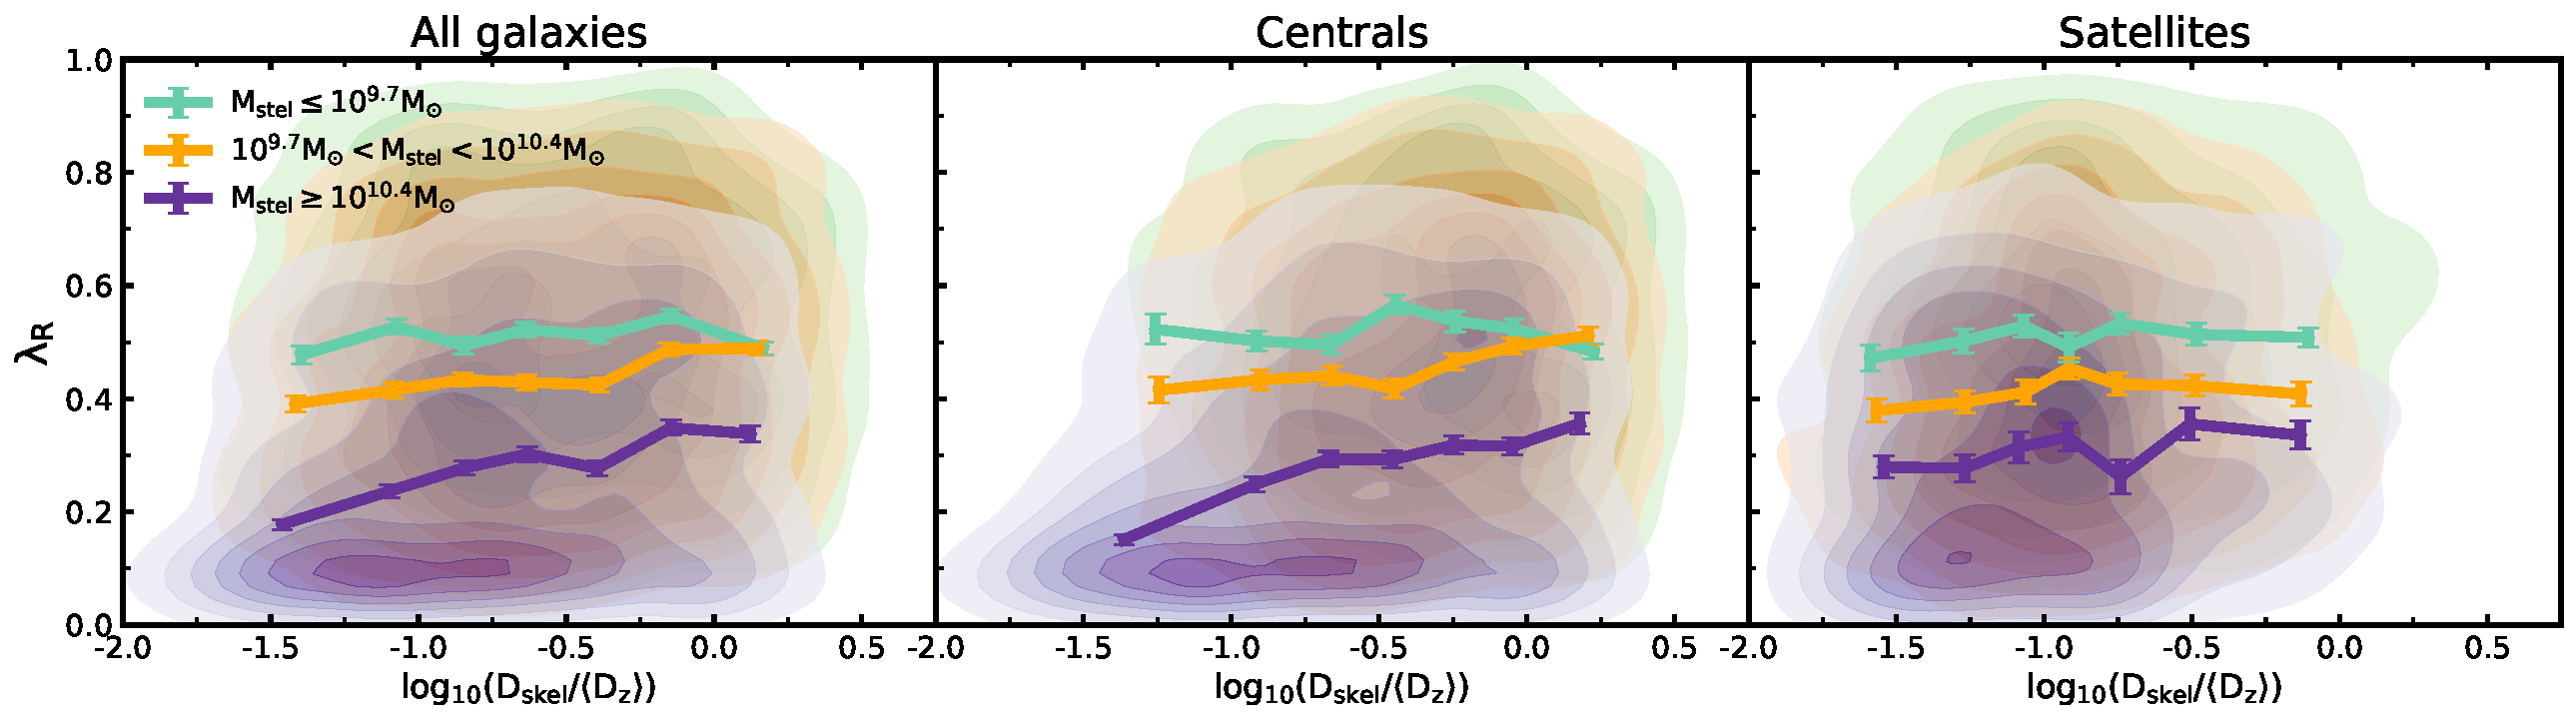
\includegraphics[width=\linewidth]{thesis/latex/cw_spin/lambdaR_dskel_mass_split_3sigma.pdf} \\
    \centering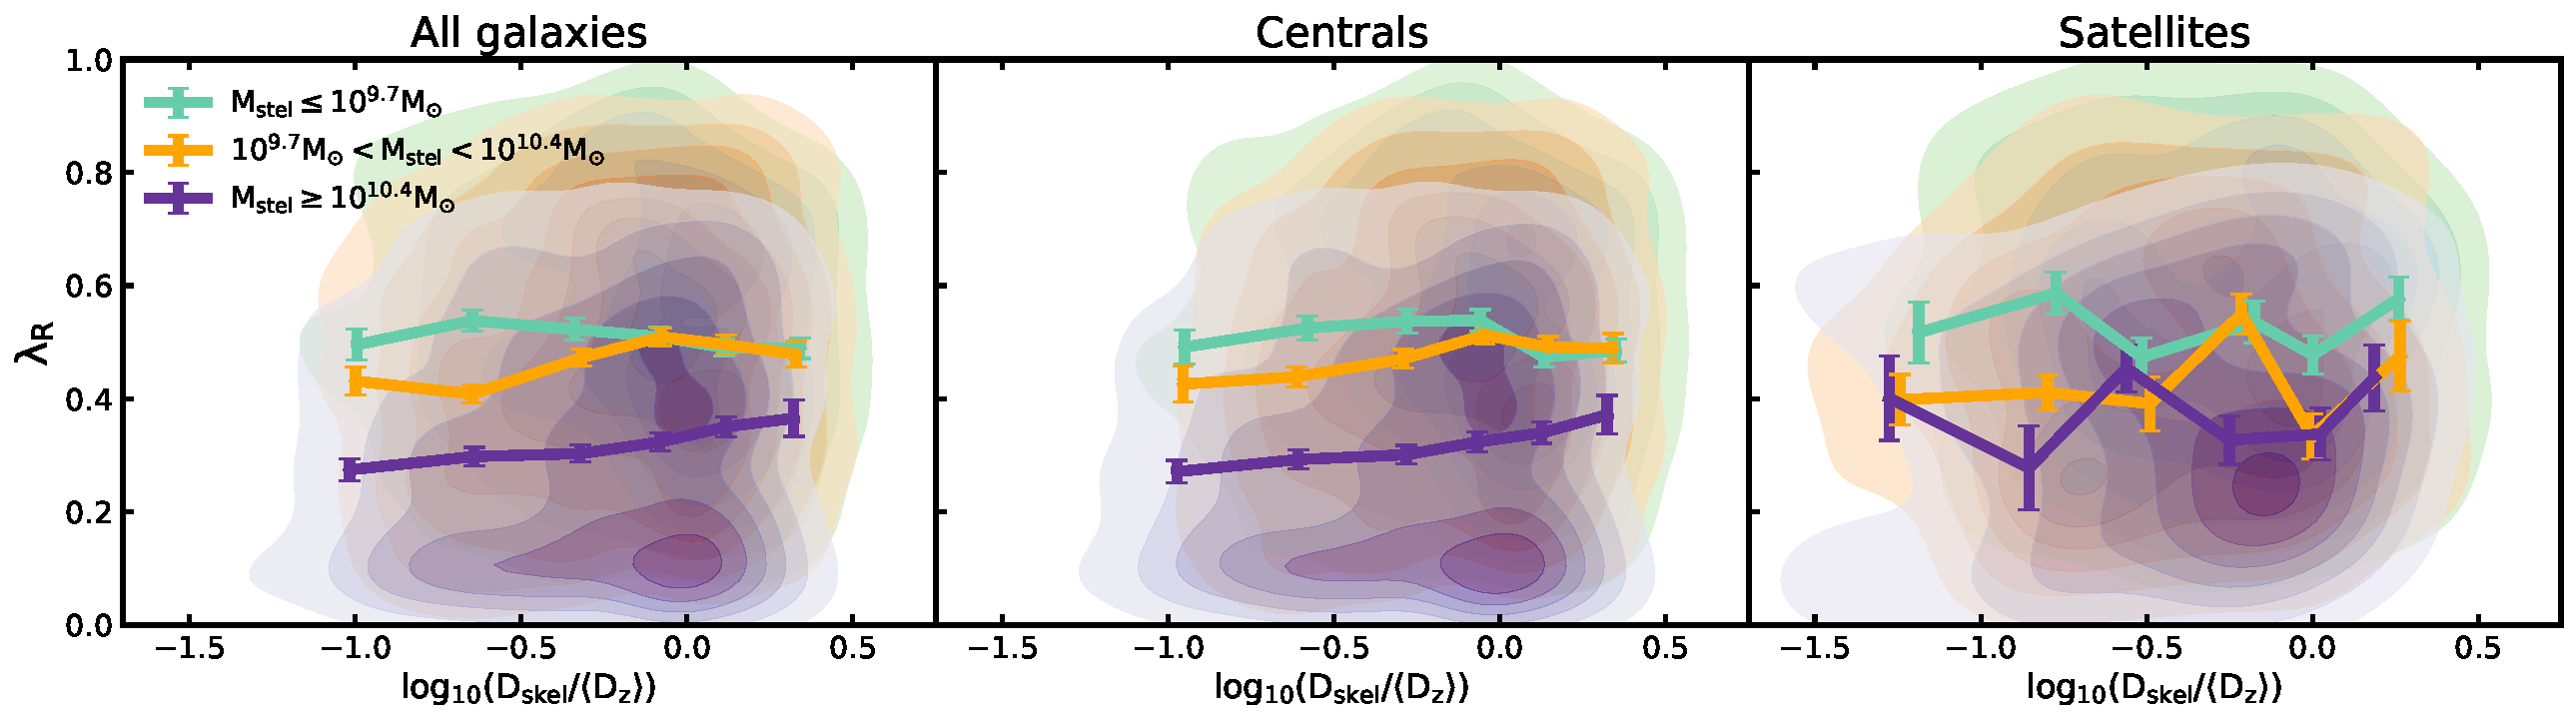
\includegraphics[width=\linewidth]{thesis/latex/cw_spin/lambdaR_dskel_no_node_mass_split_3sigma.pdf}
    \caption{Distribution of stellar angular momentum ($\mathrm{\lambda_R}$) as a function of distance to filaments ($D_{skel}$). The top row shows the distribution for all galaxies, whereas the bottom row shows the distribution now removing all galaxies close to nodes ($D_{node} < 1$Mpc). In each panel the overall distribution for three mass bins; $\mathrm{M_{stel} \leq 10^{9.7} M_{\odot}}$, $\mathrm{10^{9.7}M_{\odot} < M_{stel} < 10^{10.4}M_{\odot}}$, $\mathrm{M_{stel} \geq 10^{10.4}M_{\odot}}$ (green, orange and purple respectively) are shown by the contours using a KDE (see text), with average $\mathrm{\lambda_R}$ values shown in bins of $D_{skel}$. For the low bin, there is no particular trend with vicinity to filaments, however, the high mass bin does decrease in spin for those closer to nodes (perhaps a slight trend with the middle bin). This trend appears to be driven by centrals and is still apparent (albeit less significant) after removing those close to nodes.}
\label{fig:lambdaR_dskel}
\end{figure} 

To ensure that the lower $\mathrm{\lambda_R}$ isn't due to selection effects, in the bottom row of Figure \ref{fig:lambdaR_dskel} we again consider the dependence of $\mathrm{\lambda_R}$ on $D_{skel}$, having removed all galaxies within 1Mpc of the nearest node. This should represent a conservative selection that removes the influence of nodes, and hence, shows the underlying trends with filaments. Qualitatively we find the same trends as the top row with low and intermediate mass galaxies showing no dependence on distance to filaments, whereas high mass central galaxies closer to filaments have typically lower $\mathrm{\lambda_R}$ values, albeit with less significance. This suggests that the angular momentum content of high mass central galaxies is modulated \textit{both} with vicinity to density peaks and filamentary structure. 

We now consider how $\mathrm{\lambda_R}$ is modulated by distance to different features of the cosmic web, for individual morphologies. As demonstrated in Figure \ref{fig:morph_lambdaR_mstel}, there is a clear relationship between morphology and $\mathrm{\lambda_R}$. The relationship with $\mathrm{\lambda_R}$ and the cosmic web could therefore be due to different morphologies preferentially residing at different places with respect to nodes and filaments, or, due to a decrease in $\mathrm{\lambda_R}$ at fixed morphology. In Figure \ref{fig:etg_lambdaR_skel}, we show the distribution of $\mathrm{\lambda_R}$ for ETGs only with respect to nodes (top row) and filaments (bottom row). Due to reduced sample size, we now only separate at the median stellar mass for the population ($\mathrm{M_{stel} = 10^{10.5}M_{\odot}}$). 

Central ETGs show a slight signal for $D_{node}$ and $D_{skel}$ with decreased $\mathrm{\lambda_R}$ in closer vicinity to both. This, however, is unclear for individual mass bins and can only be seen when consider the ETG population as a whole (i.e. black line). This is consistent with the trends seen for the high mass sample in Figures \ref{fig:lambdaR_dnode} and \ref{fig:lambdaR_dskel}, albeit, with lesser significance. This suggests that the signal may be predominately driven by the spatial distribution of different morphologies (i.e. ETGs are more common closer to nodes and filaments), however, the slight evolution of $\mathrm{\lambda_R}$ at fixed morphology indicates multiple effects at play. Satellite ETGs are mostly consistent with a flat evolution with respect to both nodes and filaments. Due to lack of galaxies, we don't include the same $D_{skel}$ plot with galaxies $D_{node} < 1$Mpc removed, however, this is consistent with a flat distribution for both centrals and satellites.

\begin{figure}
    \centering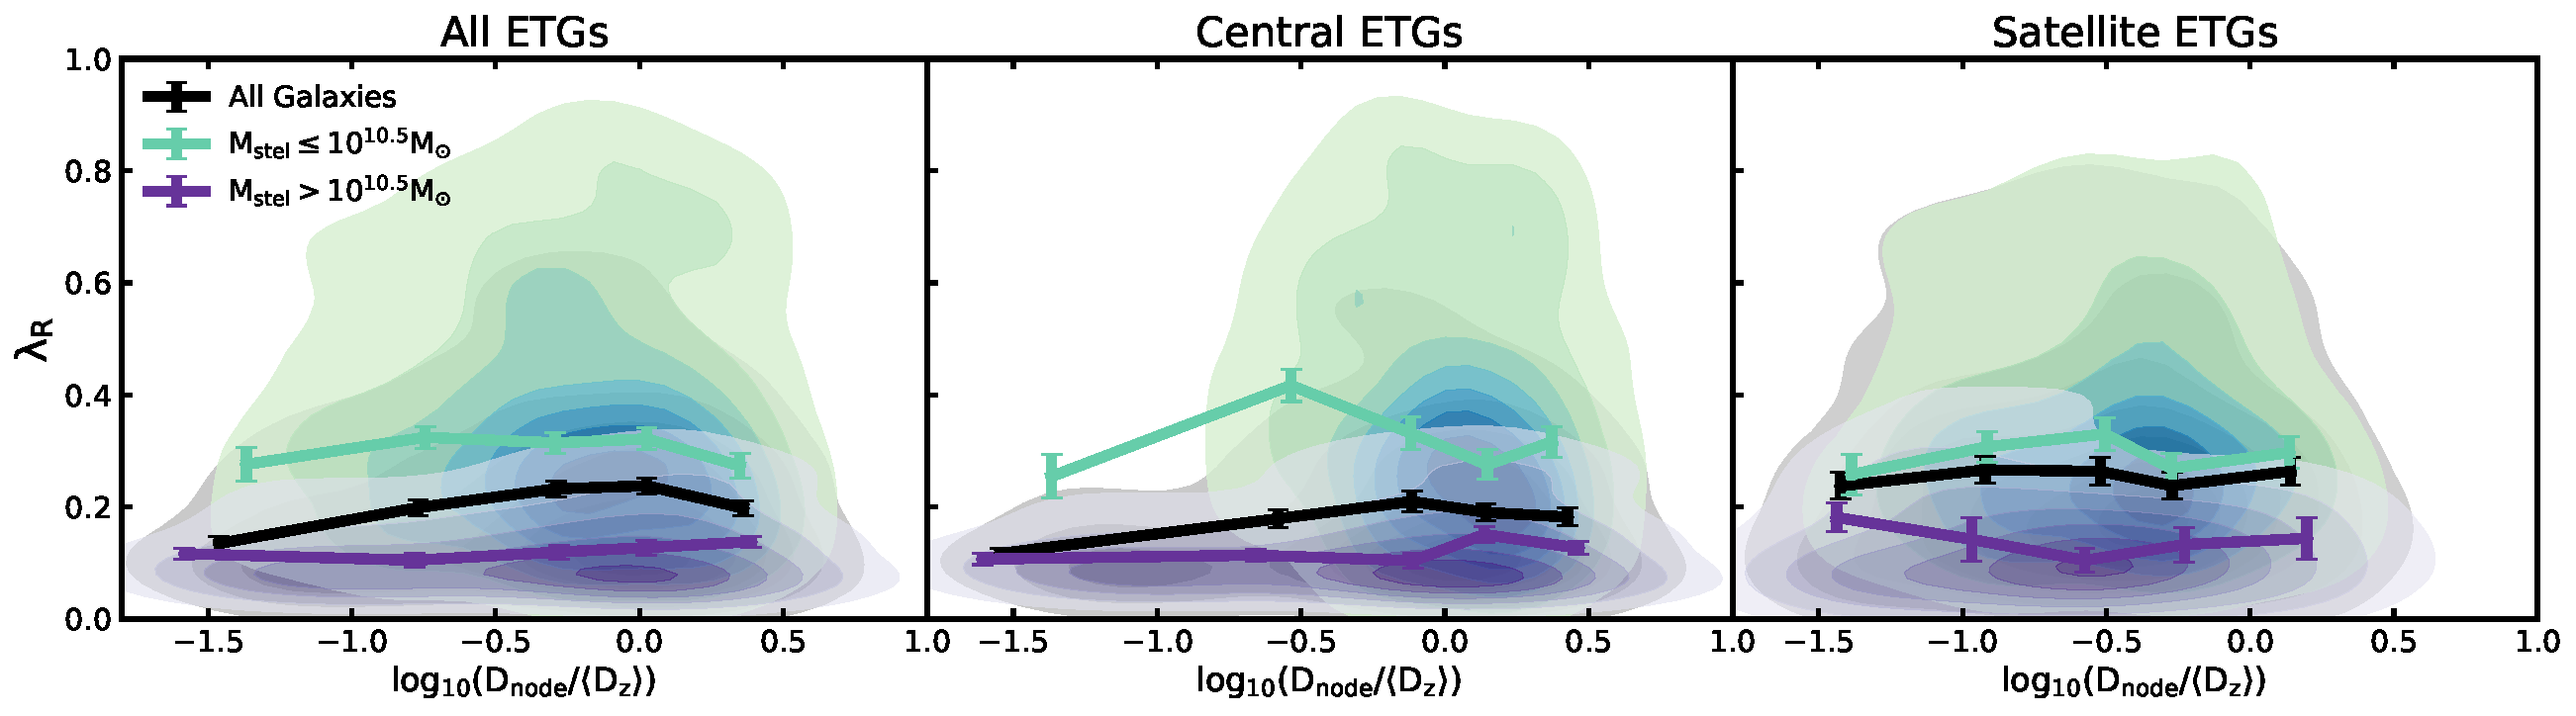
\includegraphics[width=\linewidth]{thesis/latex/cw_spin/etg_lambdaR_dnode_mass_split_3sigma.pdf} \\
    \centering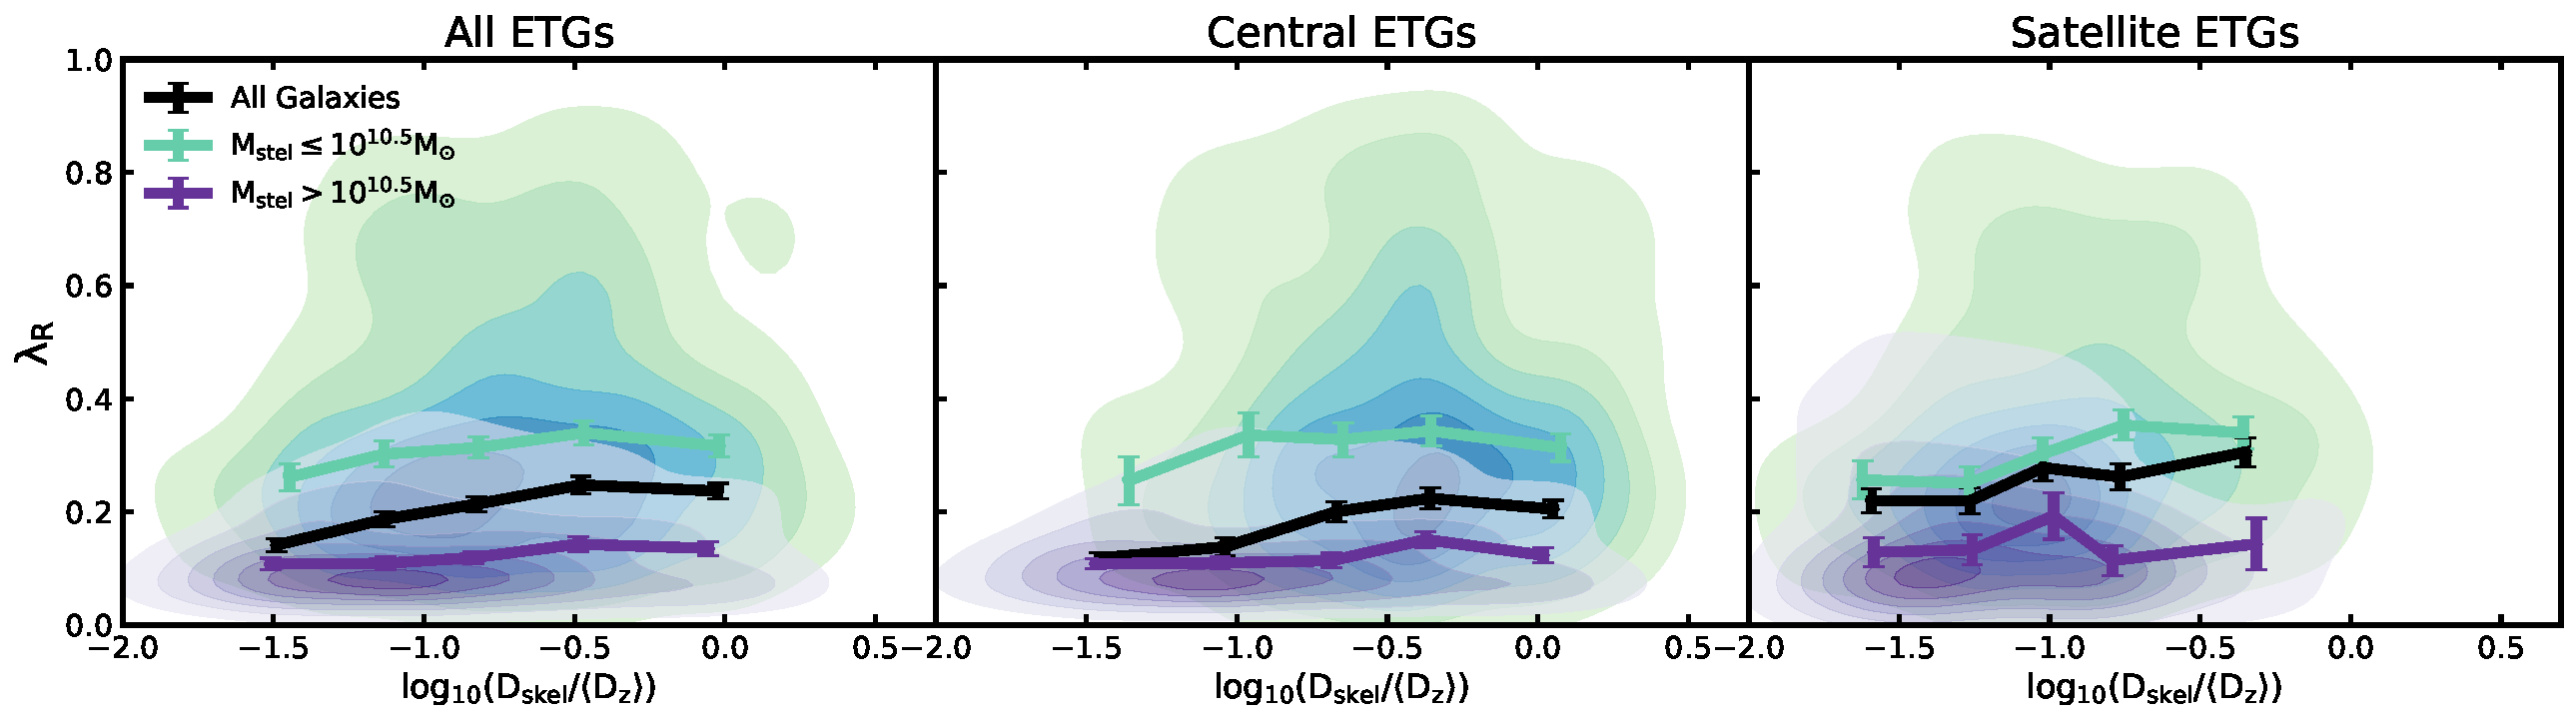
\includegraphics[width=\linewidth]{thesis/latex/cw_spin/etg_lambdaR_dskel_mass_split_3sigma.pdf}
    \caption{Distribution of stellar angular momentum ($\mathrm{\lambda_R}$) as a function of distance to nodes (top row; $D_{node}$) and filaments (bottom row; $D_{skel}$) for early-type galaxies. In each panel the population is split on the median stellar mass for ETGs ($\mathrm{M_{stel} = 10^{10.5}M_{\odot}}$). The individual distributions for the low mass (turquoise) and high mass (purple) are shown by the contours using a KDE (see text), with average $\mathrm{\lambda_R}$ values shown in bins of $D_{node}$ ($D_{skel}$). For nodes, overall we find little $\mathrm{\lambda_R}$ evolution for ETGs. We see a slight decrease in $\mathrm{\lambda_R}$ at low $D_{node}$ for central ETGs. We find a more distinct trend for ETGs with respect to $D_{skel}$; ETGs spin slower closer to filaments.}
\label{fig:etg_lambdaR_skel}
\end{figure} 

In Figure \ref{fig:ltg_lambdaR_skel}, we now show the distribution of $\mathrm{\lambda_R}$ for LTGs (i.e. everything with a disk: S0-Sds) with respect to nodes (top row) and filaments (bottom row). For each panel we split on the median stellar mass ($\mathrm{M_{stel} = 10^{10}M_{\odot}}$). Central LTGs closer to both nodes and filaments also show a slight decrease in $\mathrm{\lambda_R}$, corroborating that at fixed morphology, galaxies spin down closer to cosmic structure (albeit weakly). This appears to be driven by high mass LTGs, with low mass central LTGs and all satellite LTGs appearing to be agnostic to cosmic environment. 

\begin{figure}
    \centering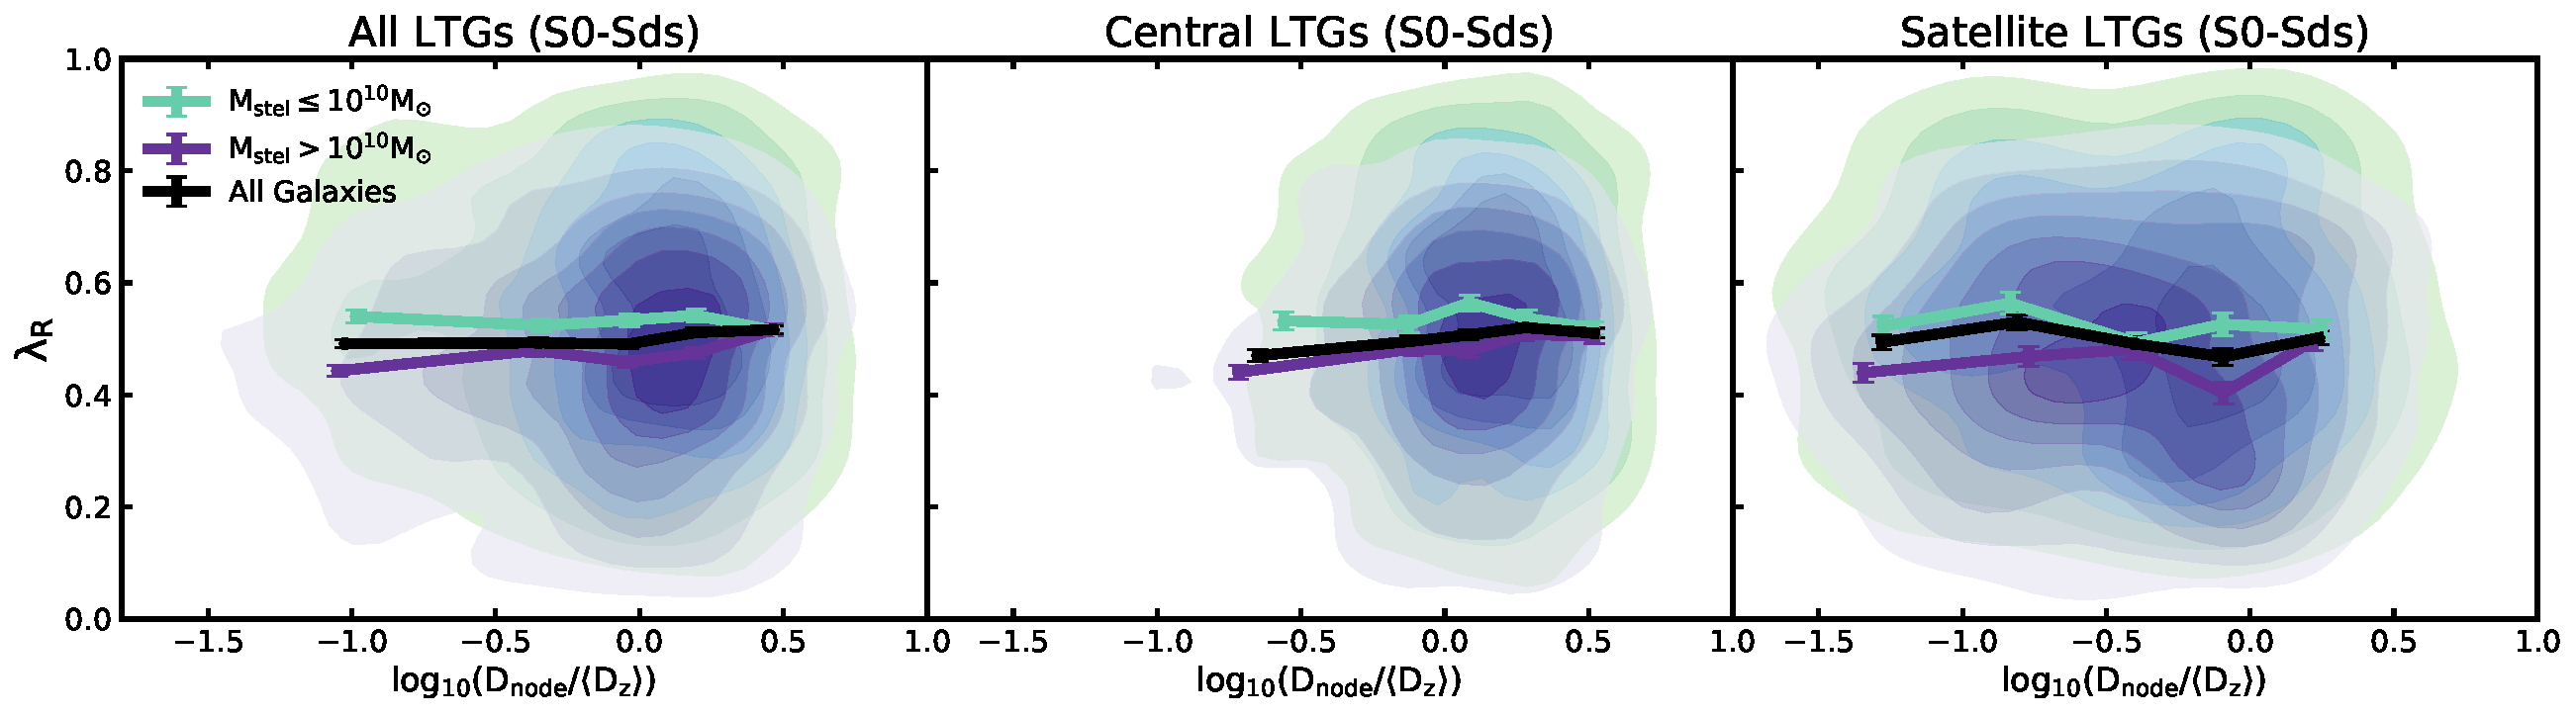
\includegraphics[width=\linewidth]{thesis/latex/cw_spin/ltg_lambdaR_dnode_mass_split_3sigma.pdf} \\
    \centering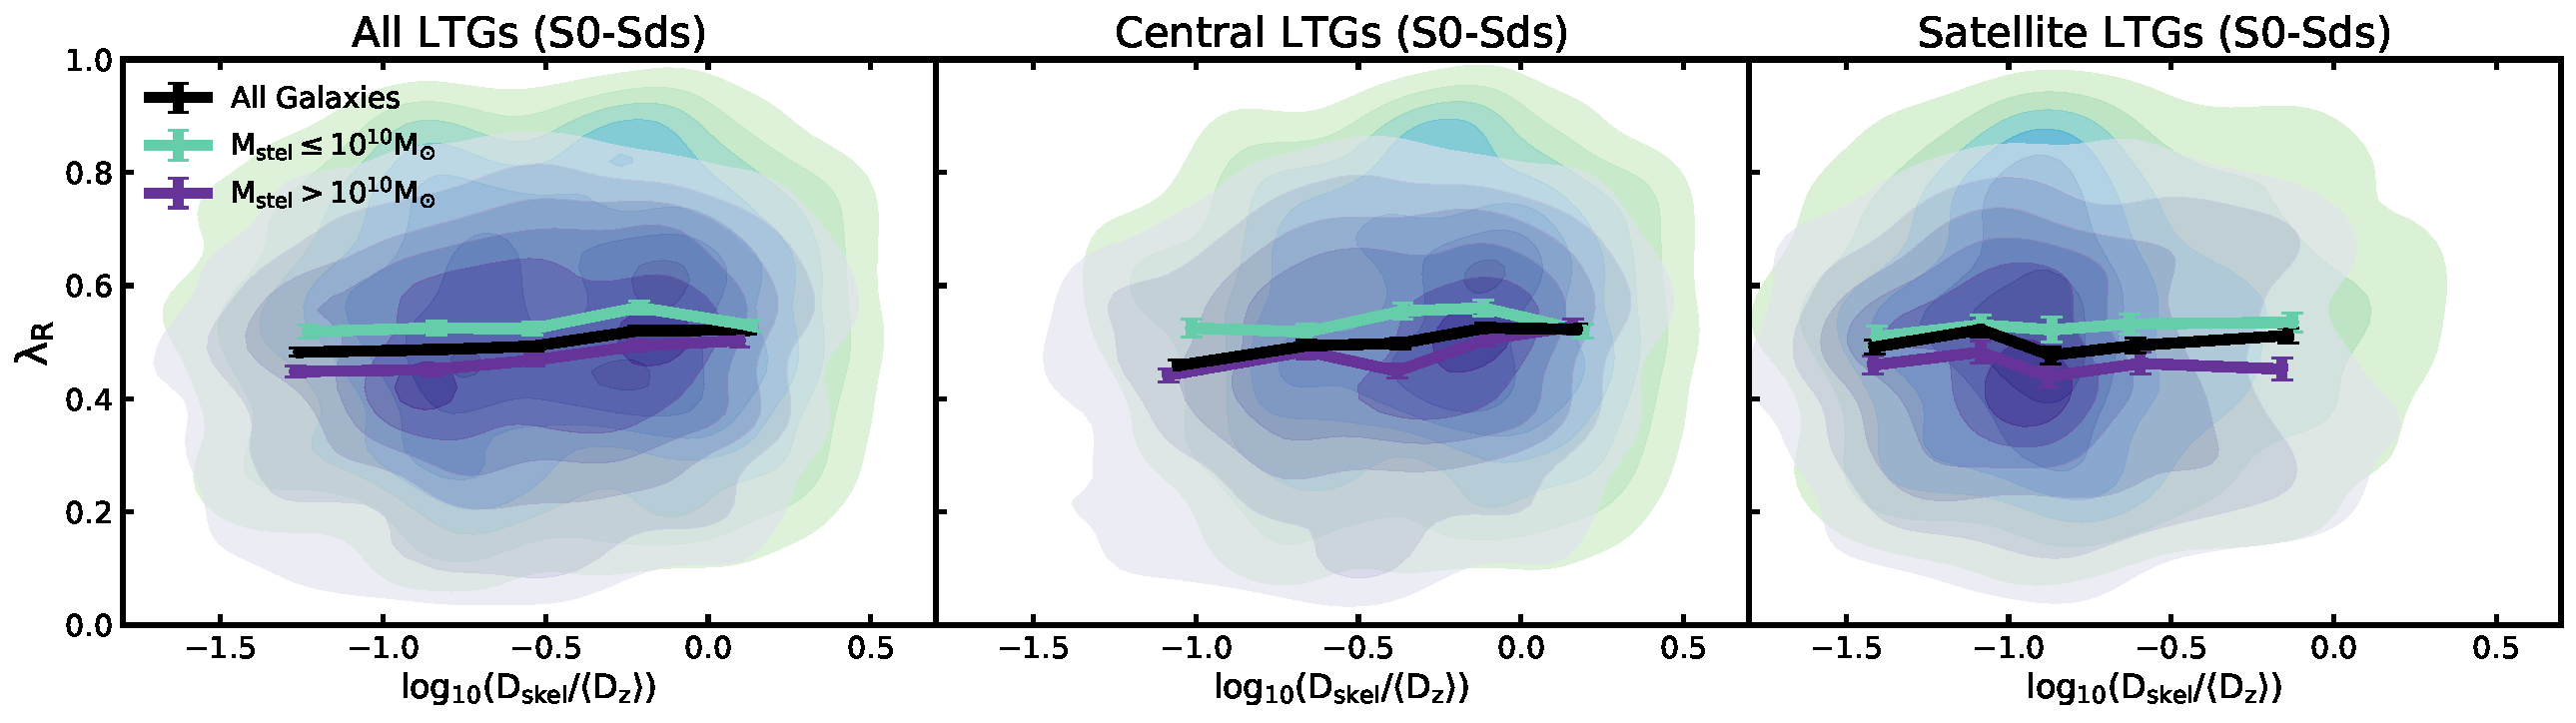
\includegraphics[width=\linewidth]{thesis/latex/cw_spin/ltg_lambdaR_dskel_mass_split_3sigma.pdf}
    \caption{Distribution of stellar angular momentum ($\mathrm{\lambda_R}$) as a function of distance to nodes (top row; $D_{node}$) and filaments (bottom row; $D_{skel}$) for late-type galaxies (i.e. S0-Sds). In each panel the population is split on the median stellar mass for LTGs ($\mathrm{M_{stel} = 10^{10}M_{\odot}}$). The individual distributions for the low mass (turquoise) and high mass (purple) are shown by the contours using a KDE (see text), with average $\mathrm{\lambda_R}$ values shown in bins of $D_{node}$ ($D_{skel}$). For central LTGs we find slight trends (driven by the low mass bin) with reduced $\mathrm{\lambda_R}$ with respect to nodes and filaments respectively. Satellite LTGs appear to agnostic to cosmic web features.}
\label{fig:ltg_lambdaR_skel}
\end{figure} 

\subsection{Discussion}
Due to tight relationship between $\mathrm{\lambda_R}$ and $\mathrm{M_{stel}}$, these result are likely in-keeping with previous findings from single fibre studies. In \citet{kraljic2018}, the relationship between distances to nodes and filaments (defined using the exact same cosmic web definitions as here) and galaxy properties such as $u - r$ colour, specific star formation rate (sSFR) and stellar mass. They find that galaxies closer to both nodes and filaments are typically more massive, redder and hosting lower star formation rates. Combining this with our findings, (central) galaxies closer to both nodes and filaments appear to undergo morphological transformation, losing angular momentum in the process (i.e. Figures \ref{fig:lambdaR_dnode} and \ref{fig:lambdaR_dskel}). This could be a natural result of over-density, as density increases going from void environments to filaments to nodes. Galaxies in more over-dense environments are naturally more likely to undergo mergers, which may in turn lower angular momentum and increase stellar mass. However, our findings that the angular momentum of satellites (at fixed mass) are agnostic to both vicinity to nodes and filaments suggest that their $\mathrm{M_{stel}}$ entirely encodes their expected $\mathrm{\lambda_R}$. 

This angular momentum loss for high mass galaxies close to filaments potentially can be understood in the context of spin \textit{alignment} (i.e. the expectation from theory that low mass disk dominated galaxies are expected to align with the neighbouring filament, whereas higher mass galaxies have perpendicular alignment). In this framework galaxies could undergo mergers along the direction of the filament (i.e. the direction of matter flow) leading to a reorientation of angular momentum to the plane of the merger, which in turn lowers the magnitude. These galaxies will now likely be higher mass and centrals. Conversely lower mass disk galaxies (typically satellites) remain unperturbed from their initial tidal field and hence have their spin direction still aligned. In theory, the spin of low mass haloes (and galaxies) embedded within filaments remain aligned due to the \textit{vorticity} from the filament leading to spin acquisition from this large-scale coherence of motion \citep[e.g.][]{pichon2011,laigle2015, codis2015}. Our findings suggest that the spin acquisition for low mass galaxies is independent regardless of their vicinity to large-scale filamentary structure (see Figure \ref{fig:lambdaR_dskel} and low mass bin of Figure \ref{fig:ltg_lambdaR_skel}). This could suggest that the scale of filamentary structure (since DisPerSE only gives the distances to the largest structures when recovering from galaxy distributions), is unimportant for the build up of angular momentum for lower mass galaxies.

We note, however, that morphology does not appear to \textit{completely} encode how spin magnitude is modulated by the cosmic web. In Figure \ref{fig:ltg_lambdaR_skel}, we find that high mass central LTGs are at typically lower spin when closer to nodes and filaments, and, the same for all central ETGs in Figure \ref{fig:etg_lambdaR_skel}. The decrease in $\mathrm{\lambda_R}$ at \textit{fixed morphology}\footnote{Noteably S0-Sds is a broad morphology category and possibly allows for some morphological evolution.} indicates that $\mathrm{\lambda_R}$ provides additional information over morphology alone. In the following section, we now investigate how spin \textit{alignment} (with respect to the filaments of the cosmic web) is modulated by morphology and $\mathrm{\lambda_R}$. 

\section{Spin alignment of spiral and S0 galaxies in MaNGA} \label{sec:spin_alignment}
Historically, exploring the relationship between the spin direction of galaxies and large scale structure has been difficult. Without spatially resolved spectra of galaxies, we are reliant on projected shapes, which introduce degeneracies with respect to the actual spin vector direction \citep[e.g. see Fig 2. in][for example of degeneracies that can occur]{motloch2020}. Due to this, and the different approaches to re-constructing the cosmic web, studies are often conflicting in findings \citep[e.g. spiral galaxies having parallel vs perpendicular orientations with respect to the cosmic web][]{tempel2013a, tempel2013, lee2007, jones2010, zhang2015}. These differences due to the reconstruction of the cosmic web can likely be explained due a difference in chosen scales. In hydrodynamical simulations, the transition mass from preferential parallel alignment to perpendicular alignment is very much dependent on the scale of the filamentary structure, such as width \citep{ganeshaiahveena2019, Kraljic2019flip}. Averaging over an ensemble of filamentary scales will likely wash out this transition, and hence preferential alignment in either direction. 

The other half of the problem can be solved, however, by having kinematic information for a large population of galaxies. Kinematic (rotational) position angles help break the degeneracy of shape orientation, and provide more robust measures of directionality. We are now in the era of multiple IFS surveys that may observe enough galaxies to find a significant detection of spin alignment. In this section we explore the concept of spin alignment in MaNGA for spirals and S0 galaxies.

\subsection{Angular momentum directions} \label{sec:thin_disk}
In order to estimate the spin direction of our galaxy sample, we assume a thin-disk approximation according to \citet{LeeErdogdu2007}. Here we summarise the key steps in calculating the three dimensional vector. Working in spherical coordinates in the reference frame of the galaxy, the spin direction can be described as
\begin{equation}
\begin{split}
\mathrm{\hat{L}_r & = \cos i,} \\
\mathrm{\hat{L}_{\theta} & = (1 - \cos^2 i)^{1/2} \sin PA,} \\
\mathrm{\hat{L}_{\phi} & = (1 - \cos^2 i)^{1/2} \cos PA,}
\end{split}
\end{equation}
where $\mathrm{PA}$ is the position angle from the stellar kinematics and $i$ is the inclination of the galaxy, defined as such
\begin{equation}
\mathrm{\cos^2 i = \frac{(b/a)^2 - p^2}{1 - p^2},}
\end{equation}
where $b/a$ is the sky projected axis ratio and $p$ is the intrinsic flatness of the galaxy \citep[varies as a function of morphology as described in][]{haynes1984}. $p$ accounts for the fact that the disk of galaxies has a finite thickness, and the presence of a bulge impacts the estimation of $b/a$. In this work we adopt an intermediate value (0.158), however choosing more extreme proposed values (0.1 - 0.23) does not change our findings. The value of $i$ is set to $\pi/2$ if $b/a < p$.

The spin direction can then be transformed into equatorial Cartesian coordinates as follows:
\begin{equation}
\begin{split}
    \hat{L}_x & = \hat{L}_r \sin \alpha \cos \beta + \hat{L}_{\theta} \cos \alpha \cos \beta - \hat{L}_{\phi} \sin \beta \\
    \hat{L}_y & = \hat{L}_r \sin \alpha \sin \beta + \hat{L}_{\theta} \cos \alpha \sin \beta + \hat{L}_{\phi} \cos \beta \\
    \hat{L}_z & = \hat{L}_r \cos \alpha - \hat{L}_{\theta} \sin \alpha
\end{split}    
\end{equation}
where $\alpha = \pi/2 - {\rm dec}$ and $\beta = {\rm RA}$. For each galaxy we also compute kinematic position angles for both the stellar and ionized gas velocity fields. We calculate position angles as described in \S\ref{sec:kin_mis}.

\subsection{LTGs}
To compute the spin direction of each galaxy in our sample, we assume a thin disk approximation (see \S\ref{sec:thin_disk}) and therefore we require each galaxy to have a well defined disk component. Overall this requires a more precise definition of morphology than used in other work in this thesis. To select a \textit{pure} spiral galaxy sample we take all objects that have a debiased vote fraction of $\geq 0.9$ for answers positive to the galaxy having a disk in GZ2. 

\begin{figure}
    \centering
    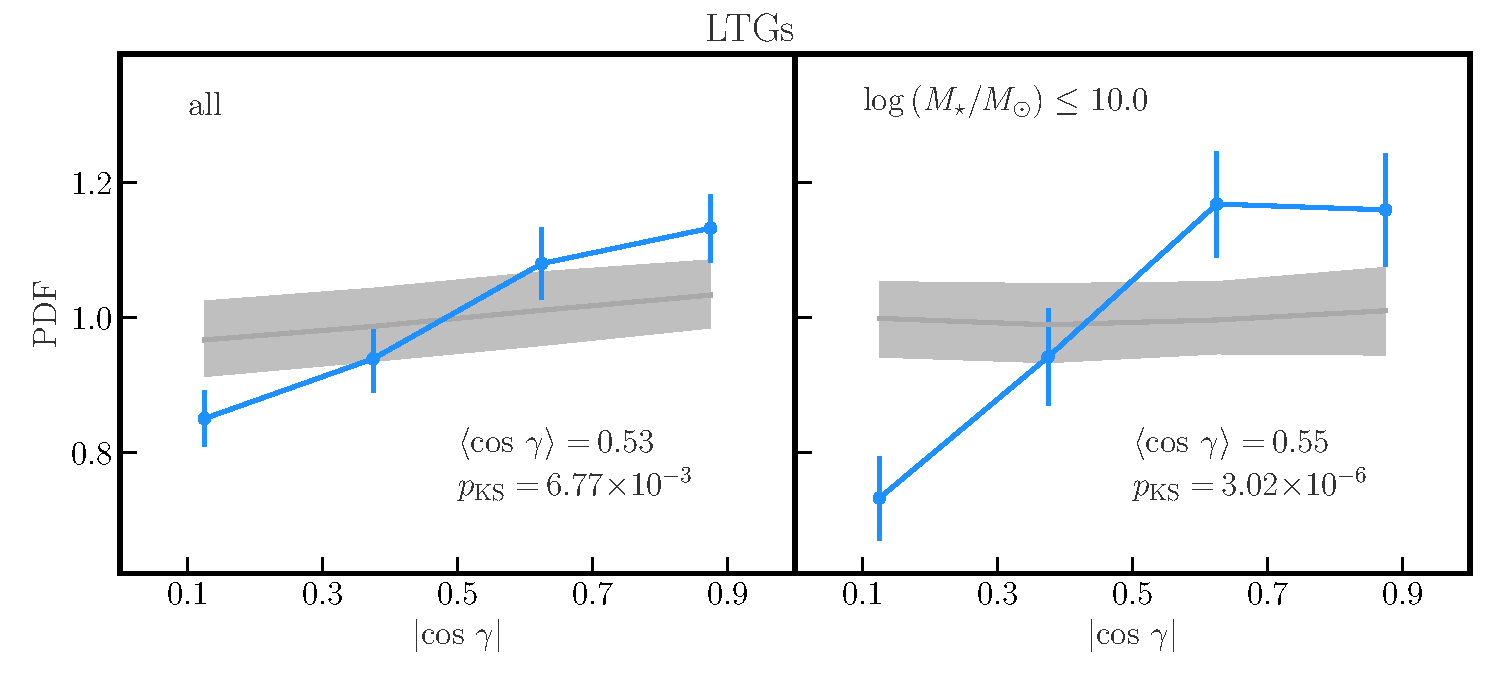
\includegraphics[width=0.65\linewidth]{thesis/latex/cw_spin/spin_fil_LTGs_2in1.pdf}
    \caption{Alignment between neighbouring filament and spin direction of late type galaxies calculated from the thin disk approximation. Each panel shows the probability density distribution (blue) of the cosine angle between the direction of the filament segment and the spin direction. Errors are calculated through bootstrapping and the solid gray line and shaded area represent the median and 95 per cent confidence limits from 2000 random samples, respectively. In addition, each panel shows the mean $\cos \gamma$ for the population and the $p$-value for a Kolmogorov--Smirnov test. The top panel shows for all LTGs in our sample, whereas the bottom panel shows the distribution only for those with a stellar mass $< 10^{10} M_{\odot}$. We find that for all masses LTGs are preferentially \textit{parallel} orientated with respect to the neighbouring filament, with low mass showing a more significant alignment signal, which appears to be driving the overall signal. We also show the alignment signal for misaligned galaxies ($\Delta$PA > 10 in this instance; blue dotted line top panel), which is consistent with the overall population.}
    \label{fig:ltgs_spin_alignment} 
\end{figure}

In Figure \ref{fig:ltgs_spin_alignment}, we show the probability density function of alignment between the spin directions of LTGs and their neighbouring filament segment. We define $\gamma$ as the angle between the spin direction and segment directions. The PDF is presented as $|\cos \gamma|$ so that 0 corresponds to exact perpendicular alignment and 1 exact parallel alignment. Each panel shows the distribution for LTGs (blue) with associated bootstrap errors, along with the expectation of the distribution if the spin vectors have completely random orientations (grey line with errors). This is implemented by fixing the galaxy positions (with respect to the filaments and their corresponding directionality) and shuffling the spin directions for the sample. In addition, each panel shows the mean $\cos \gamma$ for the population and the $p$-value for a Kolmogorov--Smirnov (KS) test between the LTGs and the random orientations. A KS test evaluates if two sub-populations are drawn from the same distribution with the null hypothesis that they are consistent. A low $p$-value therefore signifies that the populations are independent to the significance level stated. 

In the top panel, we show the orientations for all LTGs selected in our sample. We find that the spin of LTGs are preferentially orientated \textit{parallel} to the direction of the neighbouring filament segment, to the significance level of $p_{KS} = 6.19 x 10^{-3}$. We also select kinematically misaligned LTGs ($\Delta$PA > 10$^{\circ}$ in this instance due to sample size; blue dotted line) and find no appreciable difference from the overall sample. In the bottom panel, we show the PDF for only LTGs that have a stellar mass of $\mathrm{M_{stel} < 10^{10} M_{\odot}}$. Again we find a preferential parallel alignment, however, now to an increased significance level of $p_{KS} = 4.6 x 10^{-6}$. In addition $\langle \cos \gamma \rangle$ increases from 0.53 (all LTGs) to 0.55 (low mass LTGs), indicative that this signal is strongest for the low mass LTGs. This parallel alignment is in-keeping with theoretical expectation that the formation of low mass disks tend to align with the large-scale tidal field in which they evolve. 

\subsection{S0s}
To gain a more precise definition of S0s (than used previously in this thesis), we no longer use the empirical formula of GZ2 (which broadly catagories into S0-Sas). Eyeballing reveals clear spiral structure and arms for several galaxies in the S0-Sa sample, certainly Sa or later. To overcome this, we also use morphological classifications based on the the Deep Learning (DL) scheme introduced in \citet{Dominguez2018}; here we give a quick outline. The algorithm is trained on two visually-based morphological catalogues; citizen science project GZ2 and expert classifications of \citet{nair2010}. Morphology is defined for each MaNGA galaxy using SDSS photometry. The DL algorithm estimates a morphological T-type \citep[e.g. see;][for more information]{nair2010} which is first used to separate each galaxy into ETGs and LTGs. To select lenticulars, all ETGs are assigned a probability of being S0 ($P_{S0}$) based on the presence of disk structure and dominance of the bulge. To select S0 galaxies we consider all ETGs (T-type $\leq$ 0) with $P_{S0}$ > 0.5, in-keeping with \citet{Dominguez2018}. All DL classifications are finally eye-balled to check for reliability. After sample construction, our own eye-balling reveals that the ML S0 is a much cleaner sample than the GZ2 (broader) lenticular definition. Outside of intrinsic performance differences in the algorithms, this is possibly a result of the GZ2 being naturally a more broad category than the ML or that the additional eye-balling plays a role.

\begin{figure}
    \centering
    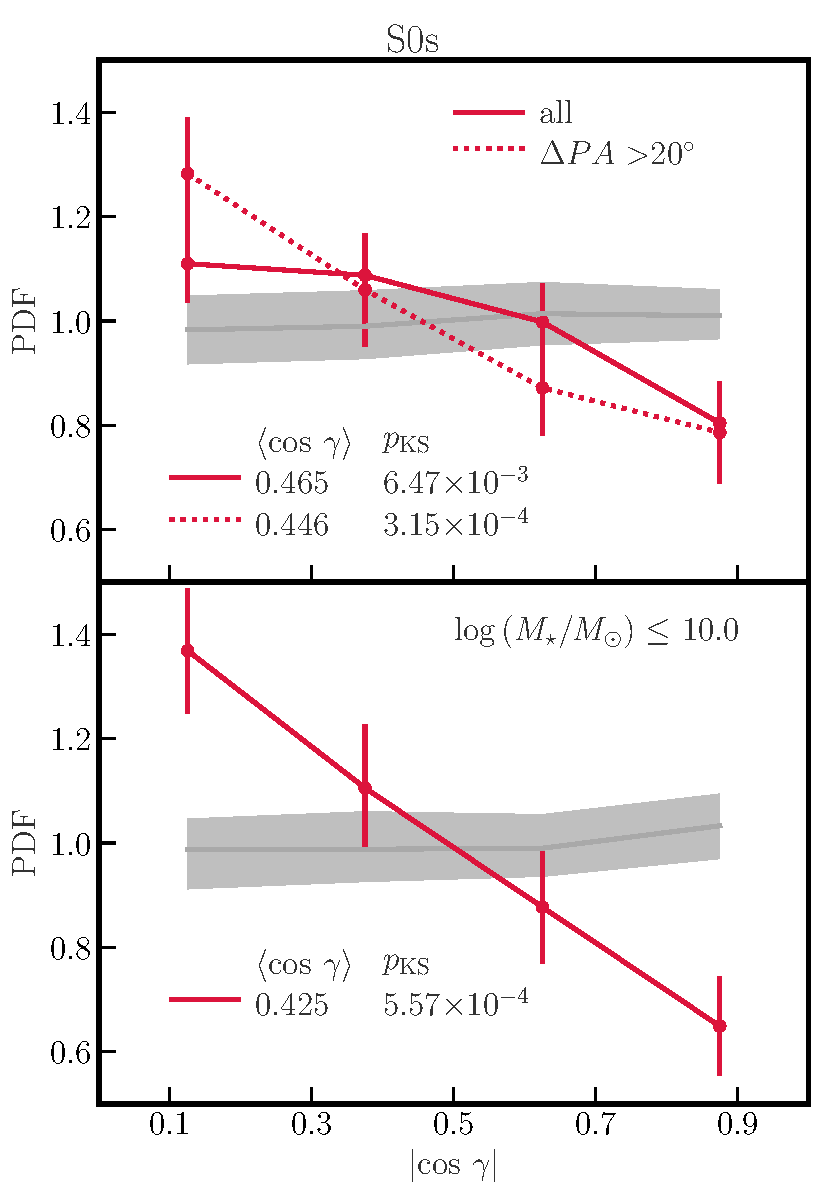
\includegraphics[width=0.65\linewidth]{thesis/latex/cw_spin/spin_fil_S0s_2in1.pdf}
    \caption{Alignment between neighbouring filament and spin direction of lenticular galaxies calculated from the thin disk approximation. Each panel shows the probability density distribution (red) of the cosine angle between the direction of the filament segment and the spin direction. Errors are calculated through bootstrapping and the solid gray line and shaded area represent the median and 95 per cent confidence limits from 2000 random samples, respectively. In addition, each panel shows the mean $\cos \gamma$ for the population and the $p$-value for a Kolmogorov--Smirnov test. The top panel shows for all S0s in our sample, whereas the bottom panel shows the distribution only for those with a stellar mass $< 10^{10} M_{stel}$. We find that for all masses lenticulars are preferentially \textit{perpendicular} orientated with respect to the neighbouring filament, with low mass showing a more significant alignment signal. We also show the alignment signal for misaligned galaxies ($\Delta PA > 20^{\circ}$; red dotted line on the top panel) which show a more significant perpendicular alignment.}
    \label{fig:s0_spin_alignment}
\end{figure}

In Figure \ref{fig:s0_spin_alignment}, we now show the PDF of alignment between the disks of lenticular galaxies and their neighbouring filament segment. As before, we show the PDF as a $\cos \gamma$ distribution with the top panel showing the results for all S0s in our sample and the bottom for low mass ($\mathrm{M_{stel} < 10^{10} M_{\odot}}$) S0s only. We also show kinematically misaligned ($\Delta$PA > 20$^{\circ}$; red dotted line top panel). Here, we find that the spin direction of S0s are preferentially \textit{perpendicular} with respect to their neighbouring filament segment. Considering the null hypothesis that the spin directions have random orientation, we find that the total S0 population is different from random to a significance of $p_{KS} = 6.47 x 10^{-3}$ which increases to  $p_{KS} = 5.57 x 10^{-4}$ when only considering the low mass S0s. On the other hand, the preferential orthogonal orientation of the spin increases for kinematically misaligned S0s ($p_{KS} = 3.15 x 10^{-4}$). This preferential perpendicular alignment could be indicative of the evolutionary history of lenticular galaxies embedded in large filamentary structure. The expectation from N-body simulations is that the orientation of dark matter haloes flip in direction due to mergers in the plane of the filament. This could be indicative that the S0s near filamentary structure have undergone mergers in their recent history, leading to a perpendicular orientation. As discussed in earlier chapters \citep[see also;][]{barrera2015, li_decoupling2019} misalignment is likely associated with mergers. The increased perpendicular alignment for the misaligned galaxies, therefore corroborates the link between spin \textit{flips} and mergers.

\subsection{Spin magnitude and alignment}
To better understand the relationship between spin magnitude and spin alignment, we now consider the alignment signal by splitting on $\mathrm{\lambda_R}$. In Figure \ref{fig:lambdaR_spin_alignment}, we now show the PDF of alignment between the disks of high spin (top row: $\mathrm{\lambda_{R}}$ > 0.73) and low spin (bottom row: $\mathrm{\lambda_{R}}$ < 0.4) galaxies. As before, we show the PDF as a $\cos \gamma$ distribution with the left panel showing the results for all galaxies in each sample and the right for low mass ($\mathrm{M_{stel} < 10^{10} M_{\odot}}$) galaxies only. 

\begin{figure}
\centering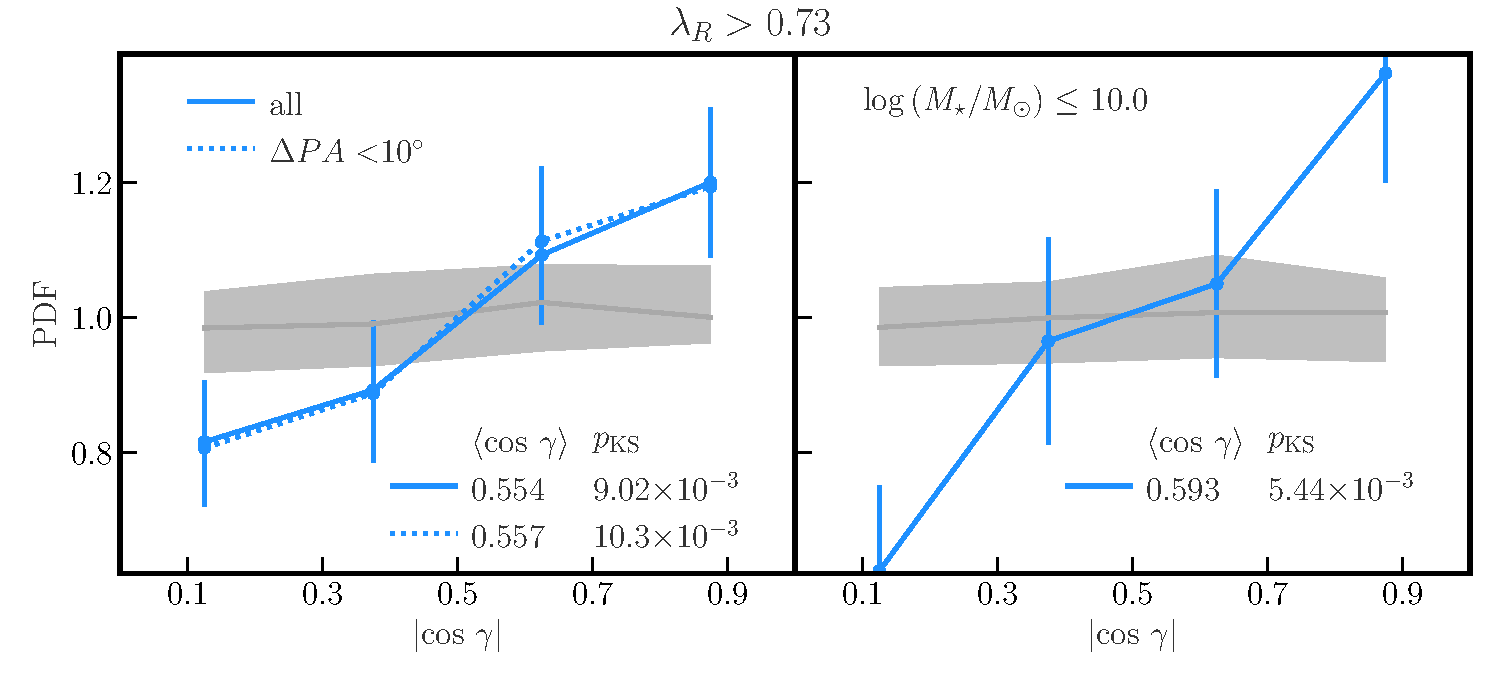
\includegraphics[width=\textwidth]{thesis/latex/cw_spin/spin_fil_high_lambdaR_2in1.pdf}\\
\centering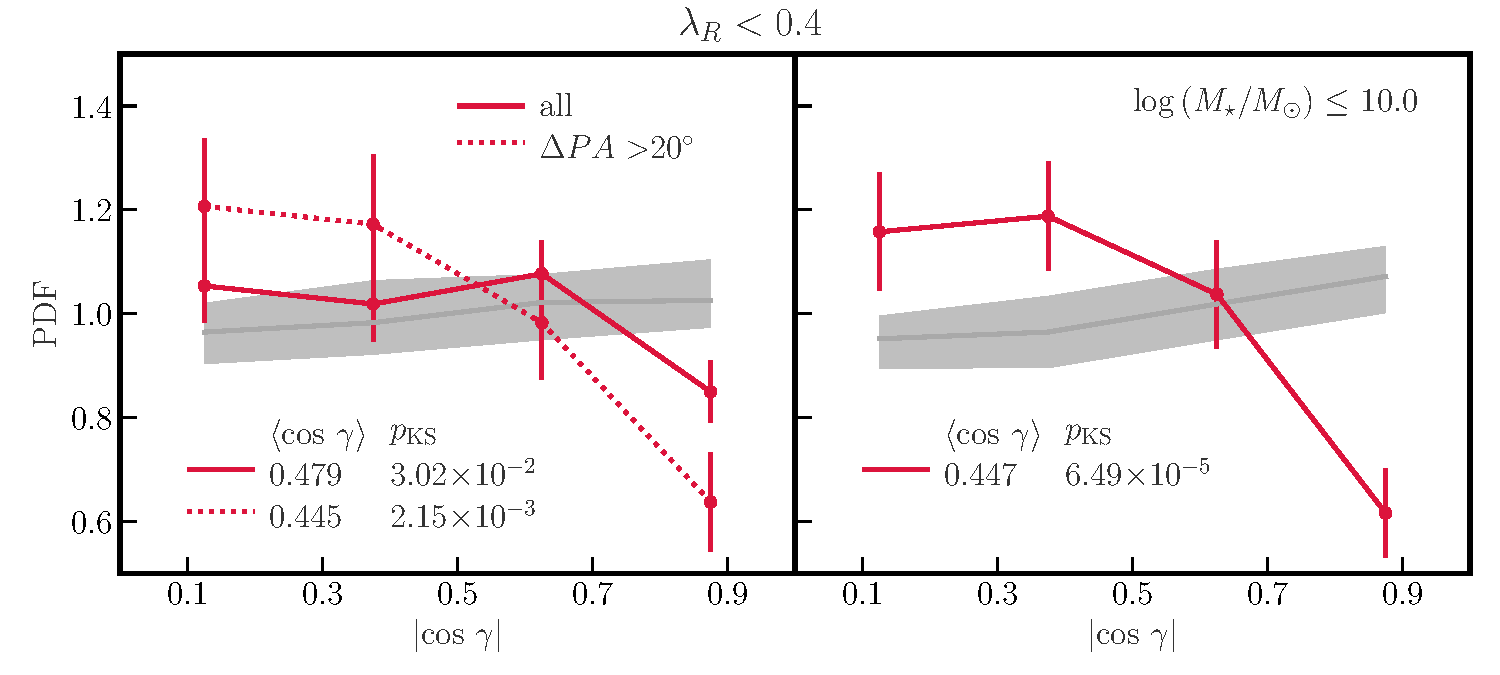
\includegraphics[width=\textwidth]{thesis/latex/cw_spin/spin_fil_low_lambdaR_2in1.pdf}
\caption{Alignment between neighbouring filament and spin direction of all galaxies calculated from the thin disk approximation split by $\mathrm{\lambda_R}$. (Top:) Alignment between the filaments and spin direction for all (left) and low-mass (right; $\mathrm{M_{stel} < 10^{10} M_{\odot}}$) galaxies with ($\mathrm{\lambda_{R}}$ > 0.73). (Bottom:) Alignment between the neighbouring filament and the spin direction for all (left) and low-mass (right; $\mathrm{M_{stel} < 10^{10} M_{\odot}}$) galaxies with ($\mathrm{\lambda_{R}}$ < 0.4). Each panel shows the probability density distribution (red) of the cosine angle between the direction of the filament segment and the spin direction. Errors are calculated through bootstrapping and the solid gray line and shaded area represent the median and 95 per cent confidence limits from 2000 random samples, respectively. In addition, each panel shows the mean $\cos \gamma$ for the population and the $p$-value for a Kolmogorov--Smirnov test. The high $\mathrm{\lambda_R}$ sample tend to have their spin parallel to their host filaments. This alignment signal appears to increase for the low mass galaxies (albeit only significantly for the outer bins). The low $\mathrm{\lambda_R}$ sample tend to have their spin oriented in a perpendicular direction with respect to the filaments. This alignment signal increases for kinematically misaligned ($\Delta$PA > 20$^{\circ}$) galaxies, and even more significantly for the low mass.}
\label{fig:lambdaR_spin_alignment}
\end{figure} 

The high $\mathrm{\lambda_R}$ galaxies demonstrate a preferential parallel alignment with respect to their host filaments. The alignment signal appears to be driven by the low mass galaxies (albeit only significantly for the outer bins). The low $\mathrm{\lambda_R}$ sample tend to have their spin oriented in a perpendicular direction with respect to the filaments. This alignment signal increases for kinematically misaligned ($\Delta$PA > 20$^{\circ}$) galaxies, and even more significantly for the low mass.

Given the typical distributions of pure LTGs (i.e. Sb-Sds) and lenticulars in the $\mathrm{M_{stel}}$, $\mathrm{\lambda_R}$ phase space (Figure \ref{fig:morph_lambdaR_mstel}), the majority of the high (low) $\mathrm{\lambda_R}$ galaxies will be pure LTGs (S0s). This result therefore reflects the previous findings with morphology. Notably, these values of $\mathrm{\lambda_R}$ were selected to maximise the spin alignment signal. Even with this selection, the significance of the preferential orientations are typically less significant than splits using morphology. This could be indicative that morphology holds a great relationship with spin alignment rather than spin magnitude. A larger sample size is, however, required to confirm this.

\section{Discussion and Summary} \label{sec:cw_spin_conclusion}
In this chapter we investigate the role of the cosmic web on galaxy kinematics, specifically the magnitude of directionality of stellar angular momentum. In \S\ref{sec:spin_magnitude} we used 8000 galaxies from the MaNGA survey to investigate how a proxy for specific stellar angular momentum (i.e. $\mathrm{\lambda_R}$) is individually dependent on stellar mass, halo mass, visual morphology, and, vicinity to different components of the cosmic web. Our key findings for this section are as follows:
\begin{itemize}
    \item Stellar angular momentum is individually dependent on both stellar mass and morphology (Figure \ref{fig:morph_lambdaR_mstel}), with higher mass galaxies typically being lower spin (for fixed morphology), and, earlier type galaxies being of lower spin than later types (at fixed mass).
    \item $\mathrm{\lambda_R}$ shows only a minimal evolution with halo mass for late-type galaxies and satellites (all morphologies), however, central ETGs in more massive groups tend to have lower angular momentum than lower $\mathrm{M_{halo}}$ (Figures \ref{fig:morph_lambdaR_mhalo} \& \ref{fig:group_membership_lambdaR}). 
    \item In general, the spin of satellite galaxies (and central galaxies $\mathrm{< 10^{10.4}M_{\odot}}$) is agnostic to their vicinity to cosmic web morphological features (i.e. nodes and filaments). High mass ($\mathrm{> 10^{10.4}M_{\odot}}$) galaxies, however, have typically lower $\mathrm{\lambda_R}$ values closer to nodes and filaments respectively (Figures \ref{fig:lambdaR_dnode} and \ref{fig:lambdaR_dskel} respectively). 
    \item When splitting on morphology, central ETGs and high mass ($\mathrm{M_{stel} > 10^{10}M_{\odot}}$ LTGs both spin down closer to nodes and filaments (Figures \ref{fig:etg_lambdaR_skel} \& \ref{fig:ltg_lambdaR_skel}). While different spatial distributions of ETGs and LTGs may account for part of the cosmic web signal, this indicates that $\mathrm{\lambda_R}$ provides additional information over morphology alone.
\end{itemize}
These results of angular momentum loss for high mass galaxies close to filaments can potentially be understood in the context of spin alignment. Galaxies undergoing mergers would be expected to (generally) have lower angular momentum amplitudes (and more likely to be higher mass and centrals). In the framework of extendend tidal tensor theory \citep{laigle2015}, these mergers could be expected to occur in the plane of the filament (i.e. direction of matter flow) leading leading to a reorientation of angular momentum to the plane of the merger (and hence perpendicular alignment). Conversely lower mass disk galaxies (typically satellites) remain unperturbed from their initial tidal field and hence have their spin direction still aligned. 

In \S\ref{sec:spin_alignment}, we investigate the 3D alignment between the spin direction of galaxy disks and their neighbouring filament. This work represents the first study using IFS data (MaNGA MPL-6; 4633 total galaxies) to estimate 3D spin directions, in the context of spin alignment. Our key findings are as follows: 
\begin{itemize}
    \item Spiral galaxies demonstrate preferentially \textit{parallel} spin orientations with respect to the nearest filament segment (Figure \ref{fig:ltgs_spin_alignment}). The significance of the alignment signal is increased if we only consider low mass LTGs ($\mathrm{M_{stel} < 10^{10} M_{\odot}}$). 
    \item Lenticular galaxies demonstrate preferentially \textit{perpendicular} spin orientations with respect to the nearest filament segment (Figure \ref{fig:s0_spin_alignment}). The significance of the alignment signal is increased if we only consider low mass S0s ($\mathrm{M_{stel} < 10^{10} M_{\odot}}$) \textit{or} those that are kinematic misaligned ($\Delta$PA > 20$^{\circ}$). 
    \item Splitting on $\mathrm{\lambda_R}$ (i.e. > 0.73 \& < 0.4) rather than morphology reveals qualitatively similar results with high (low) spin galaxies showing preferential parallel (perpendicular) alignment (Figure \ref{fig:lambdaR_spin_alignment}). 
\end{itemize}
Of most relevance to our findings are the studies of spin alignment which also make use of large scale IFS surveys. In the SAMI survey, \citet{welker2020} correlate the spin directions of galaxies estimated from kinematics with the direction of the nearest filament segment (also defined using DisPerSE). They find evidence that low mass galaxies are preferentially parallel to filaments, whereas high mass galaxies are preferentially perpendicular (to a significance of 2$\sigma$). This is in agreement with expectations of a spin \textit{flip} seen for dark matter haloes in N-body simulations, due to initial preferential alignment (for low mass haloes) with the tidal field, before mergers in the plane of the filament cause a flip in orientation. Conversely in MaNGA \citet{krolewski2019} find no evidence for spin alignment with neighbouring cosmic web structure using the vector computed from stellar velocity fields. 

In both studies the spin alignment signal is computed using the spin and filament vectors in projected 2D space. While this reduces uncertainty when reconstructing the 3D spin vector (i.e. such as making an assumption of a thin disk approximation), it does not make use of the 3D information associated with filament reconstruction. Additionally making use of only the 2D information enables studies of galaxies without disks. Projecting the angle between two 3D vectors into 2D introduces possible projection degeneracies (see black histogram in Figure \ref{fig:PA_residual}) corresponding to a standard deviation of $\sim 13^{\circ}$ from the intrinsic value. 

Parallel spin alignment between LTGs and filaments is in agreement with expectations from N-body simulations \citep[e.g.][]{laigle2015}. Our finding of perpendicular alignment for lenticulars, especially for those low mass, is perhaps more surprising. This is in direct conflict with the expectation that low mass galaxies have a parallel orientation, which flips as they grow in mass. This could be indicative that the orientation is not only a function of mass, \textit{but also of morphology.} Following the idea that lenticulars form through mergers, this could be indicative of a spin \textit{flip} at lower masses as the galaxy becomes re-orientated which is reflected in the galaxy morphology. 

We note that lenticulars (at least those selected by GZ2 in MPL-9 so not directly comparable) with $\mathrm{M_{stel} < 10^{10}M_{\odot}}$ have typically lower angular momentum than their high mass counterparts (i.e. $\mathrm{M_{stel} > 10^{10}M_{\odot}}$). This is directly the opposite to expectation of decreased $\mathrm{\lambda_R}$ with increased stellar mass seen for all other morphologies. This could corroborate the different evolutionary pathways of low mass lenticulars. We note, however, this could be a signal induced due to morphological mis-classification (i.e. low mass lenticulars are most likely to be mis-classified ETGs). The overlap in $\mathrm{\lambda_R}$ for low mass S0-Sas and ETGs in Figure \ref{fig:morph_lambdaR_mstel} could be indicative of this. In the next section, we make further use of MaNGA to explore the connection between the cosmic web and galaxy kinematics, \textit{now} in the context of halo assembly.